%-----------------------------------------------------------------------------%
\chapter{\babTiga}
%-----------------------------------------------------------------------------%

%-----------------------------------------------------------------------------%
\section{Digital Twin}
%-----------------------------------------------------------------------------%

\subsection{Konsep Digital Twin}

Digital Twin adalah representasi digital atau model virtual dari objek, proses, atau sistem fisik yang digunakan untuk mensimulasikan dan mengoptimalkan performa objek atau sistem tersebut. Konsep ini merupakan bentuk lebih maju dari simulasi tradisional dengan kemampuan mencerminkan kondisi asli atau siklus hidup dari objek fisik secara real-time, mengumpulkan data melalui sensor, dan memungkinkan analisis serta prediksi yang lebih mendalam.

% \begin{figure}[htbp]
%     \centering
%     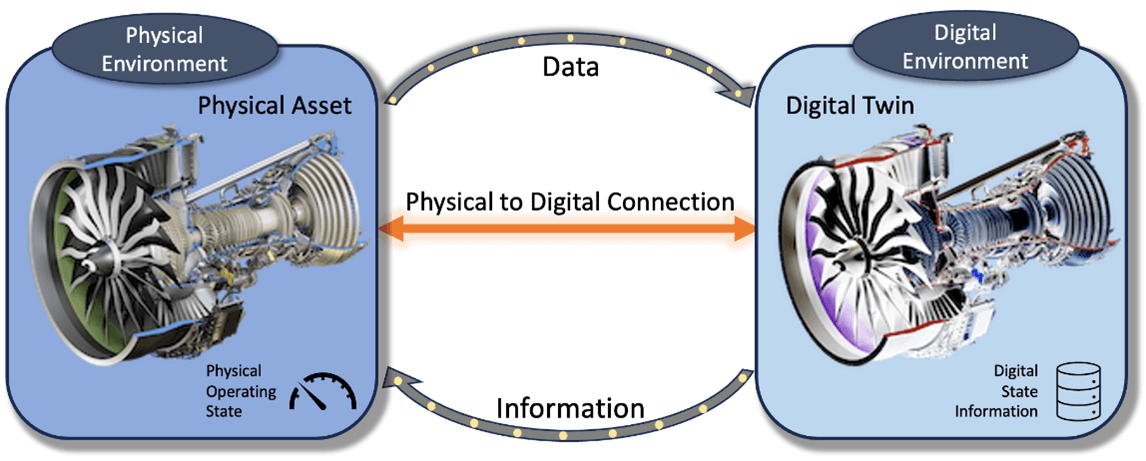
\includegraphics[width=0.8\textwidth]{assets/pics/bab3_1.png}
%     \caption{Konsep Digital Twin - Ilustrasi hubungan antara physical asset dan digital representation}
%     \label{fig:digital_twin_concept}
% \end{figure}

Digital Twin menggabungkan berbagai konsep modern seperti Internet of Things (IoT), big data, machine learning, dan artificial intelligence untuk menciptakan model digital yang digunakan. Teknologi ini dapat mereplikasi berbagai konsep barang fisik, mulai dari sebuah peralatan sehari-hari hingga instalasi besar seperti turbin angin atau bahkan sistem pembangkit energi sebuah kota.

Karakteristik utama Digital Twin ada di kemampuan sinkronisasinya secara real-time dengan objek fisik basisnya, kapabilitas analitik prediktif, dan interaktivitas dua arah antara dunia fisik dan digital. Berbeda dengan simulasi tradisional yang umumnya bersifat statis dan dijalankan dalam periode tertentu, Digital Twin beroperasi secara continuous dan terus memperbarui model berdasarkan data terbaru dari sistem fisik (selalu akurat).

\subsection{Arsitektur Digital Twin}

Arsitektur Digital Twin terdiri dari lima komponen utama yang bekerja secara sinergis untuk menciptakan representasi digital yang akurat dari unit fisik. Setiap lapisan memiliki fungsi masing-masing dalam memastikan sinkronisasi dan akurasi kerja sistem.

% \begin{figure}[htbp]
%     \centering
%     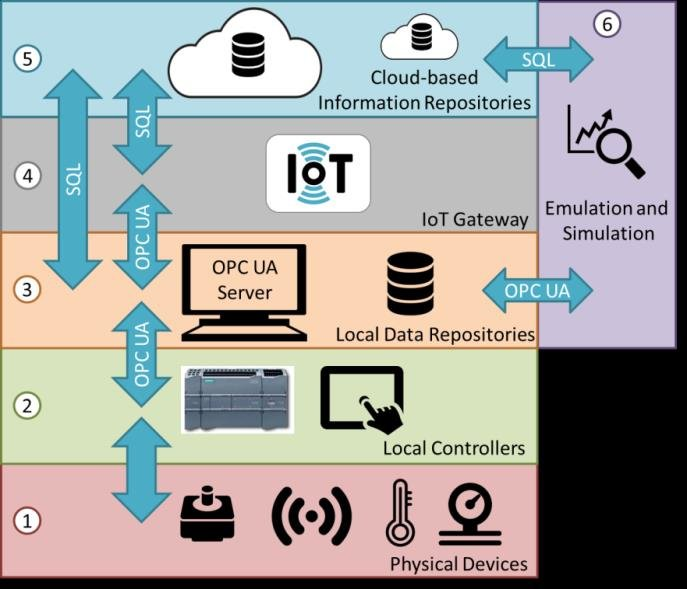
\includegraphics[width=0.8\textwidth]{assets/pics/bab3_2.png}
%     \caption{Arsitektur Digital Twin - Diagram 5 layer architecture}
%     \label{fig:digital_twin_concept}
% \end{figure}


\textbf{Lapisan Fisik (Physical Layer)} merupakan objek atau entitas real yang ingin dimodelkan, seperti mesin, bangunan, kendaraan, atau sistem jaringan. Lapisan ini adalah sumber data utama yang akan direpresentasikan secara digital. Data dari entitas asli ini kemudian dikumpulkan melalui sensor dan perangkat IoT untuk mencerminkan kondisi nyata dari objek tersebut.

\textbf{Lapisan Virtual (Virtual Layer)} adalah replika digital dari entitas fisik yang dirancang untuk mensimulasikan kondisi dan perilaku objek fisik secara dinamis. Lapisan virtual menggunakan data real-time yang dikumpulkan dari sensor untuk tidak hanya mencerminkan kondisi saat statis, tetapi juga merepresentasikan perubahan dan respons terhadap berbagai kondisi dan situasi yang dialami oleh entitas sumber data.

\textbf{Lapisan Komunikasi Data (Data Communication Layer)} berfungsi sebagai lapisan yang menghubungkan entitas fisik dengan entitas digital. Lapisan ini mencakup jaringan dan protokol yang diperlukan untuk berkomunikasi dan mentransfer data secara real-time dari sensor yang terpasang pada entitas fisik ke model digital. Keandalan dan kecepatan transfer data pada lapisan ini sangat kritis untuk memastikan bahwa model digital selalu memiliki data terkini sesuai dengan kondisi fisik yang sebenarnya.

\textbf{Lapisan Pemrosesan dan Analitik (Processing and Analytics Layer)} bertanggung jawab untuk memproses data yang dikumpulkan dari entitas fisik. Teknologi seperti big data, machine learning, dan AI digunakan untuk menganalisis data tersebut, menghasilkan prediksi, dan membuat keputusan yang tepat. Lapisan ini juga memungkinkan entitas digital untuk belajar berdasarkan data yang diterimanya untuk terus meningkatkan akurasi model machine learning.

\textbf{Lapisan Aksi dan Kontrol (Action and Control Layer)} berfungsi menerapkan hasil analisis yang dilakukan di digital twin ke dalam hasil atau aksi yang dapat dilakukan oleh entitas fisik. Lapisan ini mencakup adjustment operasional, maintenance prediktif, atau optimisasi performa. Komunikasi dari entitas digital ke entitas fisik harus dilakukan dengan cara yang aman dan real-time untuk mendapatkan respons yang akurat terhadap kondisi operasional yang direplikasi.

\subsection{Manfaat Digital Twin}

Digital Twin memberikan berbagai keuntungan signifikan dalam pengelolaan dan optimisasi sistem. Manfaat utama dari implementasi Digital Twin dapat dikategorikan ke dalam beberapa aspek operasional dan strategis.

\textbf{Simulasi dan Pengujian Tanpa Risiko} memungkinkan simulasi dan testing menyeluruh dari berbagai sistem, konfigurasi, atau skenario tanpa adanya risiko kerugian atau kerusakan sistem akibat perubahan yang tidak sesuai. Kemampuan ini mencakup pemodelan dan analisis performa sistem secara keseluruhan, identifikasi potensi munculnya masalah, dan evaluasi terhadap berbagai konfigurasi yang mungkin untuk mengoptimalkan kinerja tanpa perlu melakukan uji coba fisik yang jauh lebih mahal dan beresiko.

\textbf{Kemampuan Prediktif dan Maintenance} Digital Twin memiliki fungsi prediktif dengan memungkinkan monitoring dan analisis secara visual dan digital, lengkap dari sistem. Sensor dapat memantau output dari setiap komponen dan menandai masalah yang mungkin terjadi di masa depan untuk memprediksi failure komponen. Hal ini memungkinkan perbaikan dilakukan sebelum masalah terjadi, mengurangi downtime yang tidak terduga, dan menghemat biaya maintenance.

\textbf{Monitoring Jarak Jauh} Digital Twin memungkinkan monitoring dan pengendalian suatu fasilitas secara remote. Dengan adanya representasi virtual ini, kebutuhan untuk inspeksi langsung dapat dikurangi, terutama dalam lingkungan yang berpotensi berbahaya seperti tambang atau menara tinggi. Hal ini tidak hanya meningkatkan keamanan kerja, tetapi juga mengoptimalkan efisiensi operasional dengan meminimalkan turun tangan manual yang tidak diperlukan.

\textbf{Optimisasi Performa Real-time} memungkinkan analisis terus-menerus terhadap performa sistem dan penyesuaian parameter operasional secara dinamis. Digital Twin dapat menemukan kemungkinan optimisasi berdasarkan kondisi operasional saat ini dan sebelumnya (historis), serta memberikan rekomendasi untuk meningkatkan efisiensi dan produktivitas sistem.

\subsection{Penerapan Digital Twin dalam Jaringan}

Digital Twin telah menemukan aplikasi yang signifikan dalam domain jaringan telekomunikasi dan infrastruktur IT. Penerapan teknologi ini dalam konteks jaringan memberikan perspektif baru dalam pengelolaan dan optimisasi infrastruktur komunikasi.

\textbf{Digital Twin untuk Infrastruktur Jaringan} memungkinkan pembuatan model virtual dari komponen jaringan seperti router, switch, access points, dan server. Teknologi ini memberikan representasi real-time dari topologi jaringan, status perangkat, dan aliran trafik data. Model digital ini dapat mensimulasikan perubahan konfigurasi, upgrade perangkat, atau ekspansi jaringan sebelum implementasi pada infrastruktur fisik.

\textbf{Monitoring dan Management Jaringan} melalui Digital Twin memungkinkan administrator jaringan untuk memiliki penglihatan menyeluruh terhadap performa dan status jaringan. Sistem dapat memantau berbagai metrik seperti bandwidth utilization, latency, packet loss, dan availability dari setiap komponen jaringan. Visualisasi real-time ini membantu dalam decision-making yang lebih cepat dan akurat dalam pengelolaan jaringan.

\textbf{Prediksi dan Pencegahan Masalah Jaringan} Digital Twin dapat menganalisis pola trafik, performa lampau, dan kondisi operasional untuk memprediksi potensi masalah seperti bottleneck, kegagalan perangkat, atau degradasi performa. Kemampuan prediktif ini memungkinkan tindakan preventif yang dapat mencegah downtime dan mempertahankan kualitas layanan jaringan. Selain itu, Digital Twin dapat mensimulasikan skenario kegagalan untuk mengembangkan strategi pemulihan dan business continuity yang lebih efektif.

%-----------------------------------------------------------------------------%
\section{WiFi (Wireless Fidelity)}
%-----------------------------------------------------------------------------%

\subsection{Arsitektur WiFi}

Arsitektur IEEE 802.11 atau Wi-Fi melibatkan beberapa komponen dasar yang membentuk infrastruktur jaringan nirkabel modern. Arsitektur ini dirancang untuk menyediakan konektivitas yang lebih fleksibel dan dapat dikembangkan antara berbagai perangkat dalam lingkungan jaringan lokal nirkabel.

% \begin{figure}[htbp]
%     \centering
%     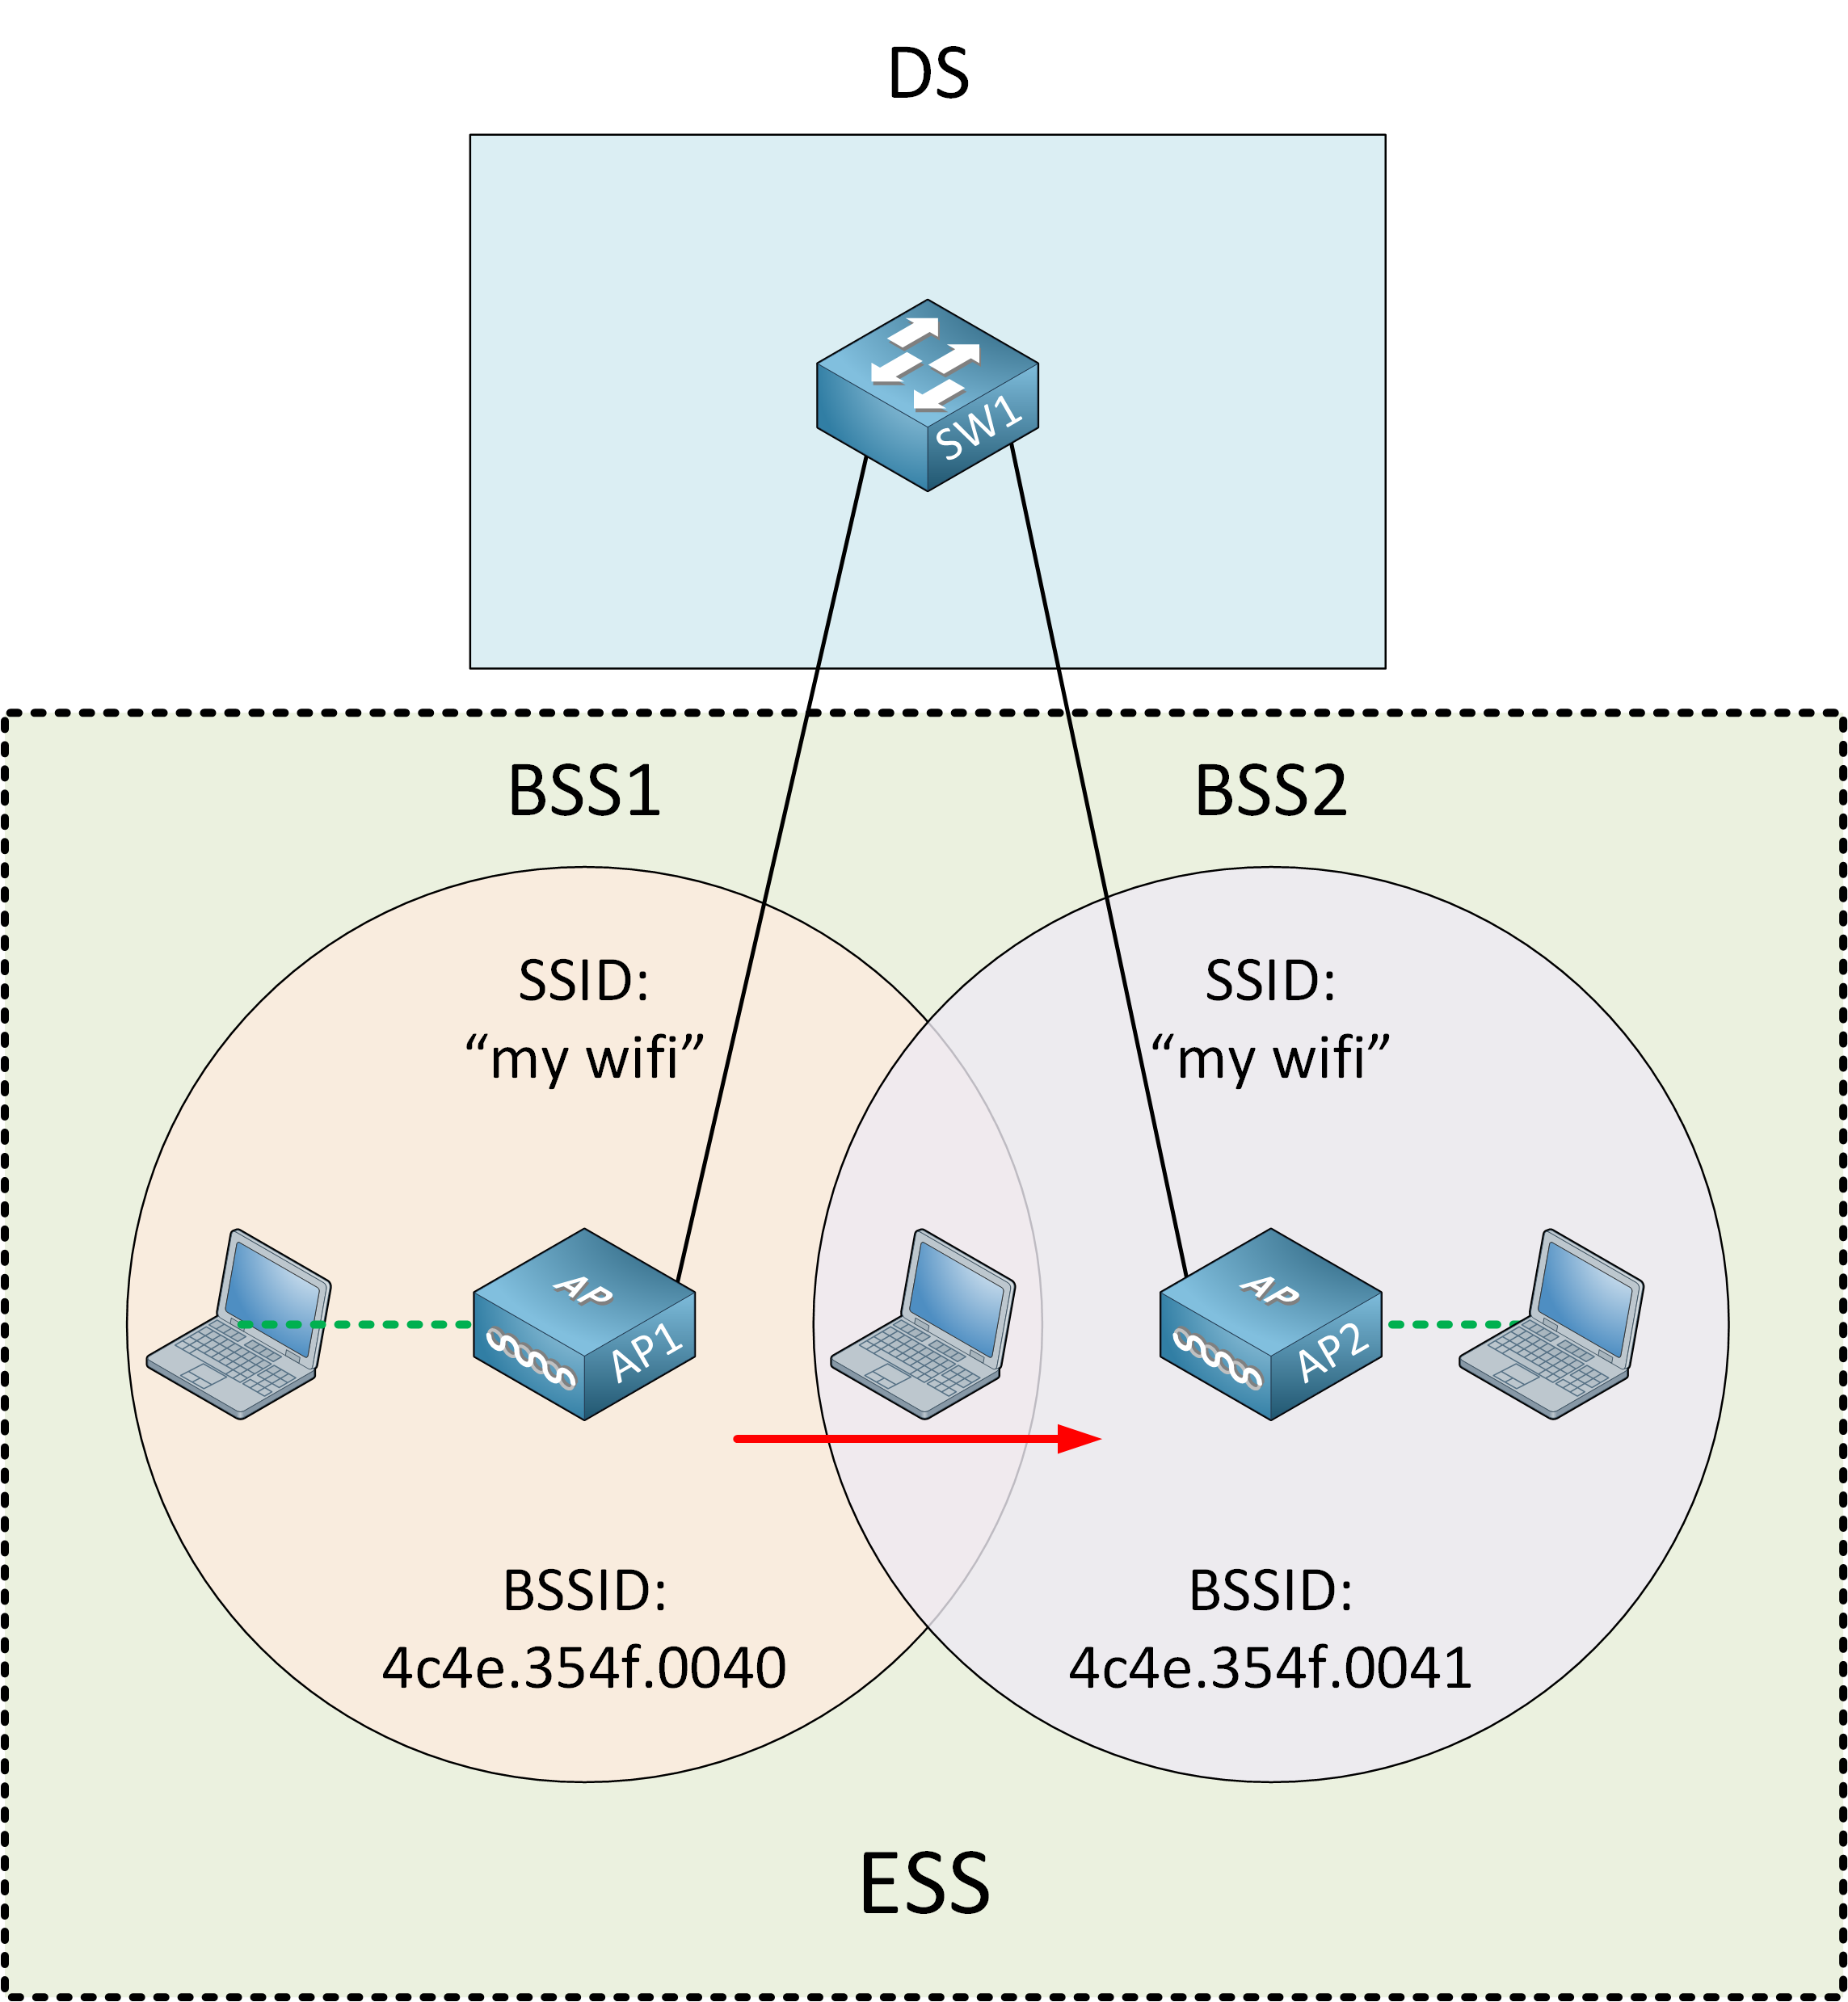
\includegraphics[width=0.8\textwidth]{assets/pics/bab3_3.png}
%     \caption{Arsitektur WiFi - Komponen dasar dari jaringan WiFi}
%     \label{fig:digital_twin_concept}
% \end{figure}

\textbf{Station (STA)} merujuk pada perangkat-perangkat yang bisa berkomunikasi menggunakan protokol IEEE 802.11. Station dapat dibagi menjadi dua jenis utama berdasarkan fungsinya dalam jaringan. Access Point (AP) berfungsi sebagai jembatan antara perangkat nirkabel dan jaringan kabel, menghubungkan station klien ke jaringan yang lebih luas dan mengatur komunikasi data antara perangkat yang terhubung. Client Station mencakup berbagai perangkat pengguna seperti laptop, smartphone, tablet, dan perangkat IoT yang membutuhkan akses jaringan melalui Access Point.

\textbf{Basic Service Set (BSS)} merupakan unit dasar dari arsitektur Wi-Fi yang terdiri dari satu Access Point dan satu atau lebih station klien yang berada dalam jangkauan komunikasi. BSS akan membentuk area layanan dasar dimana seluruh komunikasi dikoordinasikan oleh Access Point. Setiap BSS diidentifikasi oleh Basic Service Set Identifier (BSSID) yang biasanya merupakan alamat MAC dari Access Point.

\textbf{Extended Service Set (ESS)} adalah gabungan dari dua atau lebih BSS yang terhubung melalui Distribution System, memungkinkan station untuk bergerak antar BSS sambil mempertahankan konektivitas jaringan. ESS memungkinkan perpindahan yang mulus dan memperluas area cakupan jaringan Wi-Fi. Semua BSS dalam satu ESS menggunakan Service Set Identifier (SSID) yang sama.

\textbf{Distribution System} adalah infrastruktur backbone yang menghubungkan beberapa Access Point dalam satu ESS. Distribution System dapat berupa jaringan kabel Ethernet, jaringan nirkabel lainnya, atau kombinasi keduanya. Sistem ini memfasilitasi komunikasi antar BSS dan menyediakan konektivitas ke jaringan eksternal seperti internet.

\textbf{Service Set Identifier (SSID)} adalah nama jaringan Wi-Fi yang membedakan satu jaringan dari jaringan lainnya. SSID memungkinkan station klien untuk mengidentifikasi dan terhubung ke jaringan yang tepat dalam lingkungan dengan beberapa jaringan Wi-Fi. SSID dapat dikonfigurasi untuk dipancarkan secara terbuka atau disembunyikan untuk keperluan keamanan.

\textbf{Network Interface Controller (NIC)} adalah komponen perangkat keras yang memungkinkan perangkat untuk terhubung ke jaringan Wi-Fi. Wi-Fi NIC menangani proses modulasi dan demodulasi sinyal radio, implementasi protokol lapisan MAC, dan interface dengan sistem operasi perangkat untuk menyediakan layanan jaringan.

\subsection{Frekuensi dan Channel WiFi}

Wi-Fi beroperasi pada spektrum frekuensi radio yang telah dialokasikan untuk penggunaan Industrial, Scientific, dan Medical (ISM), khususnya pada pita 2,4 GHz dan 5 GHz. Karakteristik masing-masing pita frekuensi memberikan trade-off yang berbeda dalam hal jangkauan, kecepatan, dan interferensi.

% \begin{figure}[htbp]
%     \centering
%     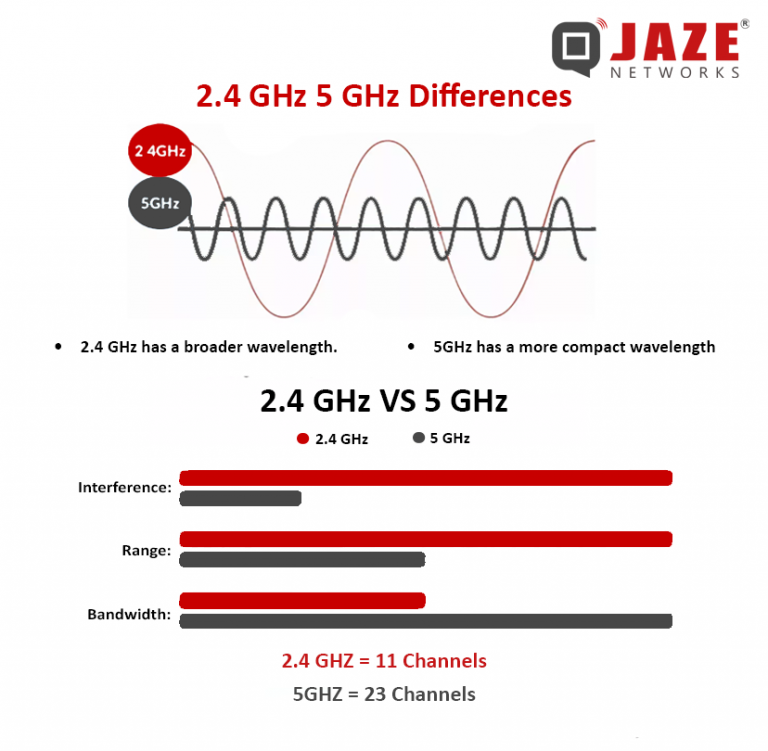
\includegraphics[width=0.8\textwidth]{assets/pics/bab3_4.png}
%     \caption{Arsitektur WiFi - 2.4 GHz vs 5 GHz}
%     \label{fig:digital_twin_concept}
% \end{figure}

\textbf{Pita 2,4 GHz} beroperasi pada rentang frekuensi 2.400-2.485 GHz dengan total bandwidth 85 MHz yang dibagi menjadi 14 channel dengan lebar 20 MHz setiap channel. Karakteristik utama pita ini meliputi propagasi yang lebih baik melalui penghalang seperti dinding dan furniture, sehingga memberikan area cakupan yang lebih luas dengan penetrasi yang superior. Namun, pita 2,4 GHz memiliki keterbatasan dalam hal jumlah channel yang tidak saling overlap yang hanya tersedia 3 channel (channel 1, 6, dan 11 di sebagian besar wilayah), yang mengakibatkan potensi interferensi yang lebih tinggi dalam lingkungan dengan banyak access point.

Pita 2,4 GHz juga menghadapi interferensi dari berbagai perangkat elektronik seperti oven microwave, perangkat Bluetooth, mouse nirkabel, dan perangkat ISM lainnya. Kecepatan data maksimum pada pita ini relatif lebih rendah dibandingkan 5 GHz, dengan throughput yang bisa menurun signifikan dalam kondisi interferensi tinggi atau kemacetan.

\textbf{Pita 5 GHz} beroperasi pada spektrum yang lebih luas dengan beberapa sub-pita: 5.150-5.250 GHz (UNII-1), 5.250-5.350 GHz (UNII-2), 5.470-5.725 GHz (UNII-2 Extended), dan 5.725-5.825 GHz (UNII-3). Total bandwidth yang tersedia mencapai 500+ MHz dengan puluhan channel yang tidak saling overlap, memberikan fleksibilitas yang jauh lebih besar dalam penerapan dan mengurangi interferensi antar channel.

Karakteristik pita 5 GHz mencakup throughput yang lebih tinggi dan latensi yang lebih rendah, namun dengan trade-off berupa jangkauan yang lebih terbatas dan penetrasi yang lebih lemah melalui penghalang. Pelemahan sinyal yang lebih tinggi pada frekuensi 5 GHz mengharuskan penerapan yang lebih padat untuk mempertahankan cakupan yang optimal.

\textbf{Alokasi dan Manajemen Channel} merupakan aspek penting dalam optimisasi kinerja Wi-Fi. Pada pita 2,4 GHz, perencanaan channel harus mempertimbangkan overlap spektrum antar channel yang berdekatan. Channel 1, 6, dan 11 adalah pilihan optimal karena tidak saling overlap dan memberikan pemisahan spektrum yang cukup. Automatic Channel Selection (ACS) dapat diimplementasikan untuk secara otomatis memilih channel terbaik berdasarkan analisis interferensi dan beban lalu lintas.

Pada pita 5 GHz, channel bonding memungkinkan penggunaan bandwidth yang lebih lebar (40 MHz, 80 MHz, atau 160 MHz) untuk meningkatkan throughput. Dynamic Frequency Selection (DFS) diperlukan pada channel tertentu untuk menghindari interferensi dengan sistem radar, yang dapat mengakibatkan perpindahan channel otomatis saat interferensi terdeteksi.

\subsection{Metrik Kinerja WiFi}

Evaluasi kinerja jaringan Wi-Fi memerlukan pemahaman terhadap berbagai metrik yang mencerminkan kualitas koneksi dan pengalaman pengguna. Metrik-metrik ini memberikan insight untuk optimisasi jaringan dan pemecahan masalah kinerja.

% \begin{figure}[htbp]
%     \centering
%     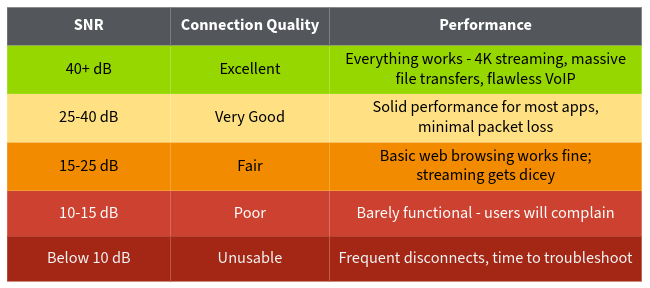
\includegraphics[width=0.8\textwidth]{assets/pics/bab3_5.png}
%     \caption{Metrik Kinerja WiFi - Dashboard menunjukkan metrik RSSI, SNR, dan throughput}
%     \label{fig:wifi_performance_metrics}
% \end{figure}

\textbf{Received Signal Strength Indicator (RSSI)} merupakan pengukuran kekuatan sinyal yang diterima oleh penerima, biasanya dinyatakan dalam satuan dBm (decibel-milliwatts). RSSI memberikan indikasi kekuatan koneksi antara klien dan access point, dengan nilai yang lebih tinggi (mendekati 0 dBm) menunjukkan sinyal yang lebih kuat. Rentang nilai RSSI umumnya berkisar antara -30 dBm hingga -90 dBm, dimana nilai di atas -50 dBm dianggap sangat baik, -50 hingga -60 dBm baik, -60 hingga -70 dBm cukup, dan di bawah -70 dBm buruk.

RSSI dipengaruhi oleh berbagai faktor termasuk jarak antara pemancar dan penerima, penghalang dan atenuasi, interferensi dari sumber lain, dan karakteristik antena kedua perangkat. Monitoring RSSI secara berkelanjutan memungkinkan deteksi degradasi sinyal dan optimisasi posisi perangkat atau access point.

\textbf{Signal-to-Noise Ratio (SNR)} mengukur rasio antara kekuatan sinyal yang diinginkan dengan tingkat noise dalam lingkungan RF. SNR dinyatakan dalam satuan dB dan merupakan indikator yang lebih akurat untuk kualitas koneksi dibandingkan RSSI saja, karena mempertimbangkan kondisi noise dalam lingkungan operasional. SNR yang tinggi (di atas 25 dB) menunjukkan kualitas sinyal yang sangat baik dengan kemampuan untuk mendukung skema modulasi dan pengkodean yang efisien.

\textbf{Throughput dan Kapasitas} merepresentasikan laju data aktual yang dapat dicapai dalam kondisi operasional nyata. Throughput efektif selalu lebih rendah dari laju data maksimum teoretis yang tercantum dalam standar, karena overhead protokol, kontesi, retransmisi, dan kondisi channel yang tidak ideal. Perencanaan kapasitas harus mempertimbangkan kebutuhan throughput total dari semua klien yang terhubung ke satu access point.

\textbf{Latensi dan Jitter} mengukur penundaan dalam transmisi data dan variasi penundaan tersebut. Latensi yang rendah (di bawah 10 ms untuk komunikasi jaringan lokal) penting untuk aplikasi real-time seperti video streaming. Jitter, atau variasi latensi, dapat mengakibatkan degradasi kualitas pada aplikasi yang sensitif terhadap konsistensi waktu.

\textbf{Area Cakupan dan Jangkauan} ditentukan oleh beberapa faktor termasuk daya pancar, gain antena, pita frekuensi, kondisi lingkungan, dan sensitivitas penerima. Perhitungan jangkauan memerlukan pertimbangan terhadap model path loss, fade margin, dan kebutuhan untuk RSSI atau SNR minimum pada area tepi cakupan.

\subsection{Manajemen dan Monitoring WiFi}

Pengelolaan jaringan Wi-Fi modern memerlukan pendekatan sistematis yang mencakup manajemen terpusat, monitoring rutin, dan optimisasi aktif. Kompleksitas lingkungan Wi-Fi enterprise dengan ratusan atau ribuan access point mengharuskan implementasi sistem manajemen yang teroptimisasi untuk mempertahankan kinerja dan reliability jaringan.
% [GAMBAR] WiFi Management Architecture - Centralized management system dengan controller dan APs

\textbf{Sistem Manajemen Terpusat} menyediakan titik kontrol tunggal untuk konfigurasi, monitoring, dan pemeliharaan seluruh infrastruktur Wi-Fi. Wireless LAN Controller (WLC) atau platform manajemen berbasis cloud memungkinkan administrator untuk mengelola ribuan access point dari satu interface terpusat. Sistem ini mendukung penerapan konfigurasi massal, pembaruan firmware, penegakan kebijakan keamanan, dan manajemen frekuensi radio terkoordinasi di seluruh jaringan.

Arsitektur terpusat juga memfasilitasi fitur-fitur canggih seperti perpindahan mulus, load-balancing, dan mitigasi interferensi yang memerlukan koordinasi antar banyak access point. Prinsip Software-Defined Networking (SDN) semakin diadopsi dalam manajemen WiFi untuk memberikan kemampuan pemrograman dan otomasi yang lebih canggih.

\textbf{Alat Monitoring Kinerja} menyediakan visibilitas waktu nyata terhadap kesehatan jaringan dan pengalaman pengguna. Solusi monitoring jaringan mengumpulkan metrik komprehensif termasuk event asosiasi/disasosiasi, kegagalan autentikasi, throughput per klien, utilisasi channel, tingkat interferensi, dan kinerja aplikasi. Platform monitoring canggih mengintegrasikan algoritma machine learning untuk deteksi anomali dan analitik prediktif.

\textbf{Teknik Optimisasi Jaringan} mencakup berbagai strategi untuk memaksimalkan kinerja jaringan Wi-Fi. Algoritma Radio Resource Management (RRM) secara otomatis mengoptimalkan assignment channel, tingkat daya pancar, dan pola cakupan berdasarkan kondisi lingkungan waktu nyata. Band steering memandu klien yang mampu dual-band untuk menggunakan pita 5 GHz ketika memungkinkan untuk mengurangi kemacetan pada 2,4 GHz.

Mekanisme load balancing mendistribusikan klien secara merata di seluruh access point yang tersedia untuk mencegah hotspot dan mempertahankan pengalaman pengguna yang konsisten. Protokol airtime fairness memastikan bahwa klien lama dengan data rate rendah tidak mendominasi waktu udara dan menurunkan kinerja untuk seluruh jaringan.

\textbf{Implementasi Quality of Service (QoS)} dalam lingkungan Wi-Fi memerlukan koordinasi antara segmen jaringan nirkabel dan kabel. Standar Wi-Fi Multimedia (WMM) menyediakan prioritas lalu lintas pada segmen nirkabel dengan empat kategori akses: Voice (\texttt{AC\_VO}), Video (\texttt{AC\_VI}), Best Effort (\texttt{AC\_BE}), dan Background (\texttt{AC\_BK}). Implementasi QoS canggih mendukung alokasi bandwidth per pengguna, traffic shaping berbasis aplikasi, dan integrasi dengan kebijakan QoS enterprise.

Adaptasi QoS dinamis dapat menyesuaikan prioritas berdasarkan kondisi jaringan dan kebutuhan aplikasi. Aplikasi real-time seperti streaming dan video conferencing memerlukan kebutuhan latensi dan jitter yang ketat yang diprioritaskan melalui mekanisme QoS.

%-----------------------------------------------------------------------------%
\section{Jaringan 5G}
%-----------------------------------------------------------------------------%

\subsection{Gambaran Umum Jaringan 5G}

Jaringan 5G atau Fifth Generation Mobile Network merupakan evolusi teknologi komunikasi nirkabel yang mengubah total skala konektivitas dan kinerja jaringan besar. Teknologi ini dirancang untuk memenuhi kebutuhan transformasi digital kecepatan yang sangat tinggi, latensi rendah, dan kemampuan konektivitas perangkat secara masif.

% \begin{figure}[htbp]
%     \centering
%     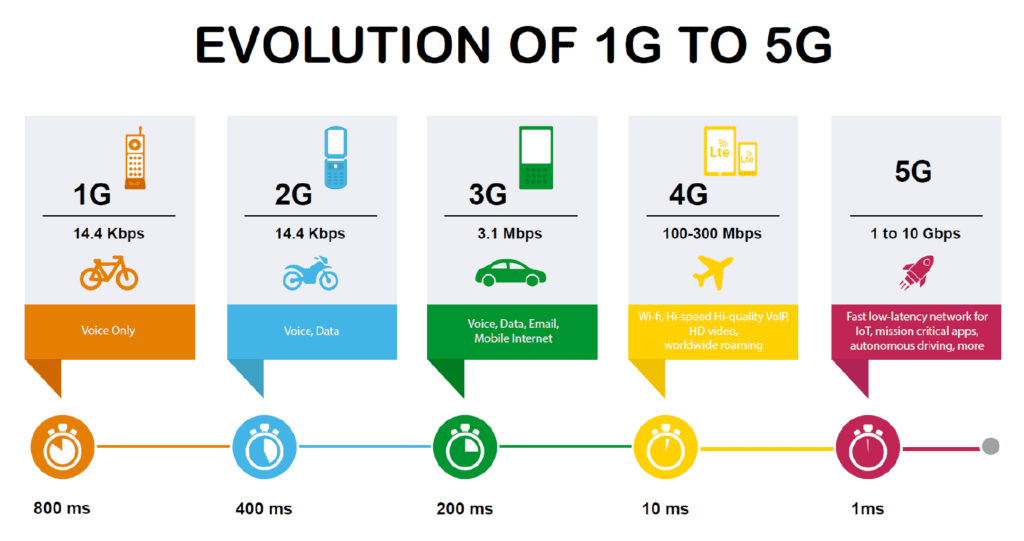
\includegraphics[width=0.8\textwidth]{assets/pics/bab3_6.png}
%     \caption{Gambaran Umum Jaringan 5G - Diagram menunjukkan arsitektur dan komponen utama 5G}
%     \label{fig:5g_overview}
% \end{figure}

Karakteristik fundamental 5G mencakup Enhanced Mobile Broadband (eMBB) yang menyediakan peak data transfer hingga 20 Gbps downlink dan 10 Gbps uplink, Ultra-Reliable Low-Latency Communications (URLLC) dengan latensi serendah 1 milidetik, dan Massive Machine-Type Communications (mMTC) yang mendukung hingga 1 juta perangkat terhubung per kilometer persegi. Kombinasi kemampuan ini memungkinkan use case  yang sebelumnya tidak memungkinkan dengan teknologi 4G/LTE.

Perbedaan signifikan 5G dengan generasi sebelumnya terletak pada arsitektur jaringan yang sepenuhnya tervirtualisasi dan cloud-native. Jaringan 5G memanfaatkan spektrum yang lebih efisien termasuk frekuensi millimeter wave, teknologi antena seperti Massive MIMO, dan kemampuan network slicing yang memungkinkan beberapa jaringan virtual pada infrastruktur fisik yang sama.

\textbf{Indikator Kinerja Utama (KPI)} 5G ditetapkan oleh International Telecommunication Union (ITU) dalam spesifikasi IMT-2020. Target maksimum transfer data 20 Gbps untuk downlink dan 10 Gbps untuk uplink, kecepatan data yang dialami pengguna minimum 100 Mbps di area perkotaan dan 50 Mbps di area pinggiran kota. Kebutuhan latensi untuk aplikasi URLLC tidak boleh melebihi 1 ms untuk user plane, sementara latensi control plane harus di bawah 10 ms.

Efisiensi spectral 5G meningkat 3x dibandingkan LTE-Advanced, kapasitas traffic area mencapai 10 Mbps per meter persegi di area hotspot, dan kepadatan koneksi mendukung 1 juta perangkat per kilometer persegi. Efisiensi energi per bit harus 100x lebih baik dari 4G, dan dukungan mobilitas hingga 500 km/jam untuk skenario transportasi berkecepatan tinggi.

\textbf{Kasus Penggunaan Utama} 5G dikategorikan dalam tiga kategori layanan utama. Enhanced Mobile Broadband (eMBB) fokus pada layanan laju data tinggi seperti streaming video 4K/8K, augmented reality (AR), virtual reality (VR), dan alat multimedia yang memerlukan throughput tinggi konsisten dan mobilitas yang mulus.

Ultra-Reliable Low-Latency Communications (URLLC) memungkinkan aplikasi kritis waktu seperti kendaraan autonomous, otomasi industri, operasi jarak jauh, dan kontrol infrastruktur yang memerlukan kinerja deterministik dan latensi rendah.

Massive Machine-Type Communications (mMTC) mendukung ekosistem IoT dengan sejumlah besar sensor terhubung, infrastruktur smart city, sistem monitoring pertanian, dan penerapan smart meter yang memerlukan daya tahan baterai yang lama dan konektivitas hemat biaya untuk aplikasi laju data rendah.

\subsection{Arsitektur Jaringan 5G}

Arsitektur 5G mengadopsi Service-Based Architecture (SBA) yang merepresentasikan perubahan fundamental dari arsitektur telekomunikasi tradisional menuju pendekatan berbasis cloud-native dan mikroservis. Arsitektur ini memungkinkan penerapan modular, penskalaan horizontal, dan inovasi layanan cepat melalui interface dan API yang terstandarisasi.

% \begin{figure}[htbp]
%     \centering
%     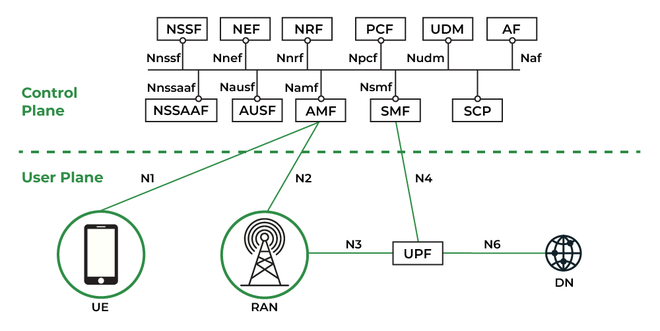
\includegraphics[width=0.8\textwidth]{assets/pics/bab3_7.png}
%     \caption{Arsitektur Jaringan 5G - Diagram menunjukkan 5GC, NG-RAN, dan interkoneksi}
%     \label{fig:5g_architecture}
% \end{figure}

\textbf{5G Core Network (5GC)} merupakan otak dari sistem 5G yang mengimplementasikan semua fungsi control plane dan user plane melalui fungsi jaringan yang virtualized. 5GC dirancang dengan prinsip cloud-native menggunakan kontainerisasi, arsitektur mikroservis, dan metodologi DevOps untuk memberikan skalabilitas, ketahanan, dan efisiensi operasional.

Service-Based Architecture dalam 5GC memungkinkan fungsi jaringan untuk saling berkomunikasi melalui Service-Based Interfaces (SBI) yang terstandarisasi lewat RESTful API dan protokol HTTP/2. Pendekatan ini memfasilitasi kebabasan / interoperabilitas vendor, pengembangan fitur yang cepat, dan komposisi layanan fleksibel berdasarkan kebutuhan kasus penggunaan spesifik.

\textbf{New Radio Access Network (NG-RAN)} mencakup semua teknologi akses radio yang terhubung ke 5GC, termasuk stasiun basis 5G NR (New Radio) (gNodeB) dan eNodeB 4G yang telah ditingkatkan untuk mendukung konektivitas 5G. Arsitektur NG-RAN mendukung berbagai skenario penerapan termasuk mode non-standalone (NSA) dan standalone (SA).

Pemisahan fungsional dalam NG-RAN memungkinkan penerapan fleksibel antara centralized unit (CU), distributed unit (DU), dan radio unit (RU) untuk mengoptimalkan kinerja, biaya, dan fleksibilitas penerapan berdasarkan kebutuhan jaringan spesifik dan kasus penggunaan.

\textbf{User Equipment (UE)} dalam konteks 5G mencakup berbagai macam perangkat mulai dari smartphone tradisional hingga sensor IoT khusus, kendaraan otonom, peralatan industri, dan perangkat augmented reality. Kategori UE 5G didefinisikan berdasarkan kemampuan dan kebutuhan kinerja untuk berbagai kasus penggunaan.

Klasifikasi UE mencakup kategori smartphone untuk layanan eMBB, kategori IoT untuk aplikasi mMTC dengan protocol stack yang disederhanakan dan daya tahan baterai yang diperpanjang, dan kategori URLLC untuk aplikasi misi-kritis yang memerlukan karakteristik kinerja deterministik.

\subsection{Fungsi Jaringan dalam 5G}

5G Core Network mengimplementasikan berbagai fungsi jaringan khusus yang menggantikan elemen jaringan tradisional dengan alternatif tervirtualisasi dan cloud-native. Setiap fungsi jaringan memiliki tanggung jawab spesifik dan berkomunikasi melalui interface yang terstandarisasi.

% \begin{figure}[htbp]
%     \centering
%     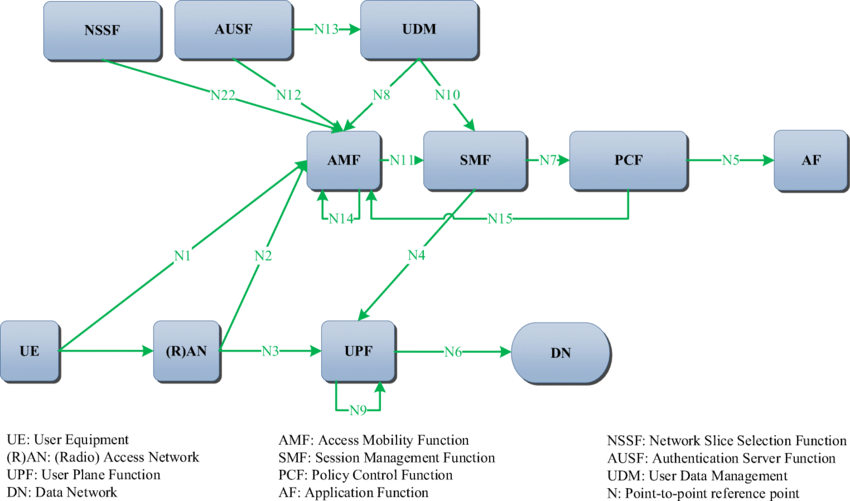
\includegraphics[width=0.8\textwidth]{assets/pics/bab3_8.png}
%     \caption{Fungsi Jaringan 5G - Diagram menunjukkan interaksi antara fungsi jaringan kunci dalam 5GC}
%     \label{fig:5g_network_functions}
% \end{figure}

\textbf{Access and Mobility Management Function (AMF)} bertanggung jawab untuk semua prosedur terkait akses dan mobilitas termasuk manajemen registrasi, manajemen koneksi, manajemen mobilitas, dan autentikasi akses. AMF juga menangani prosedur keamanan, layanan lokasi, dan koordinasi dengan fungsi kontrol kebijakan untuk penegakan kebijakan yang sesuai.

AMF mempertahankan informasi konteks UE dan koordinasi dengan Session Management Function untuk pembentukan dan manajemen sesi user plane. Dalam skenario dengan network slicing, AMF dapat mendukung beberapa slice dan memfasilitasi pemilihan slice yang sesuai berdasarkan kemampuan UE dan kebutuhan layanan.

\textbf{Session Management Function (SMF)} mengelola seluruh prosedur terkait sesi termasuk pembentukan, modifikasi, dan penghentian sesi. SMF bertanggung jawab untuk alokasi alamat IP UE, pemilihan dan kontrol fungsi user plane, pengarahan lalu lintas, dan penegakan QoS untuk sesi individual.

SMF juga mengimplementasikan fungsi pengisian, kemampuan legal eavesdropping, dan integrasi dengan kontrol kebijakan untuk penetapan policy dinamis. Dalam skenario multi-akses, SMF dapat mengelola sesi yang mencakup berbagai teknologi akses yang berbeda.

\textbf{User Plane Function (UPF)} menangani semua penerusan lalu lintas pengguna, inspeksi paket, penegakan quality of service, dan fungsi pelaporan. UPF dapat diterapkan dalam berbagai konfigurasi termasuk penerapan terpusat untuk backhaul lalu lintas atau penerapan terdistribusi untuk skenario edge computing.

Implementasi UPF canggih mendukung fitur seperti traffic directing berdasarkan identifikasi aplikasi, caching konten lokal, dan integrasi edge computing untuk aplikasi latensi ultra-rendah. UPF juga memfasilitasi integrasi dengan jaringan data eksternal dan jaringan enterprise.

\textbf{Network Repository Function (NRF)} menyediakan kemampuan penemuan layanan yang memungkinkan fungsi jaringan untuk menemukan dan berkomunikasi dengan instans layanan yang sesuai. NRF mempertahankan registri instans fungsi jaringan yang tersedia, kemampuan mereka, dan status beban saat ini untuk penyeimbangan beban yang cerdas.

NRF mendukung layanan dinamis yang penting untuk operasi cloud-native, penskalaan otomatis, dan skenario pemulihan kesalahan dalam penerapan 5GC terdistribusi.

\subsection{Network Slicing}

Network Slicing merupakan inovasi kunci dalam 5G yang memungkinkan pembuatan jaringan virtual pada infrastruktur fisik yang bisa dibagi-bagikan. Setiap slice dapat dikustomisasi untuk kebutuhan kasus penggunaan spesifik dengan sumber daya khusus, karakteristik kinerja, dan kebijakan keamanan.

% \begin{figure}[htbp]
%     \centering
%     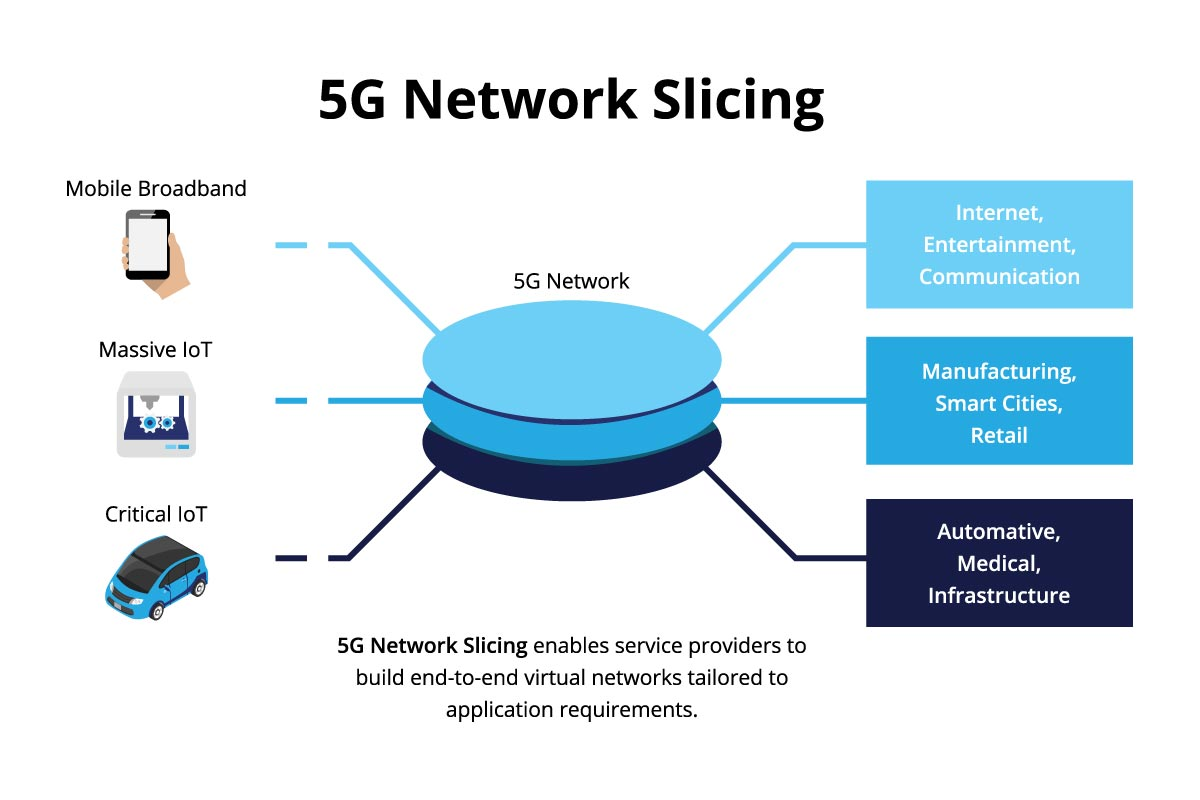
\includegraphics[width=0.8\textwidth]{assets/pics/bab3_9.png}
%     \caption{Konsep Network Slicing - Beberapa slice melayani berbagai kasus penggunaan}
%     \label{fig:network_slicing_concept}
% \end{figure}

\textbf{Konsep dan Implementasi} Network Slicing mencakup virtualisasi ujung ke ujung dari radio access network, transport network, dan core network untuk menciptakan instans jaringan yang terisolasi. Setiap slice dapat memiliki perjanjian tingkat layanan yang berbeda, kebutuhan kinerja, dan kebijakan operasional yang independen dari slice lainnya.

Instansiasi slice melibatkan manajemen fungsi jaringan yang sesuai, alokasi sumber daya, dan manajemen konfigurasi di berbagai domain teknologi. Teknologi software-defined networking dan virtualisasi fungsi jaringan memfasilitasi pembuatan dan manajemen slice secara dinamis.

\textbf{Jenis dan Karakteristik Slice} dapat dikategorikan berdasarkan kebutuhan layanan utama. Slice eMBB dioptimalkan untuk aplikasi throughput tinggi dengan penekanan pada laju data puncak dan pengalaman pengguna. Slice URLLC diprioritaskan untuk latensi ultra-rendah dan reliability tinggi dengan sumber daya khusus dan prosedur protokol yang dioptimalkan.

Slice mMTC dirancang untuk konektivitas perangkat masif dengan penekanan pada efisiensi energi, optimisasi biaya, dan prosedur yang disederhanakan untuk aplikasi IoT. Slice kustom dapat dibuat untuk kebutuhan enterprise spesifik atau kasus penggunaan khusus yang tidak tercakup oleh jenis slice standar.

\textbf{Isolasi dan Manajemen Sumber Daya} memerlukan pemisahan ketat antara slice yang berbeda untuk memastikan jaminan kinerja dan kebutuhan keamanan. Isolasi sumber daya dapat diimplementasikan pada berbagai tingkat termasuk sumber daya komputasi, penyimpanan, jaringan, dan alokasi spektrum radio.

Algoritma alokasi sumber daya dinamis dapat menyesuaikan sumber daya slice berdasarkan permintaan real-time dan kebutuhan perjanjian tingkat layanan. Platform orkestrasi canggih mendukung manajemen siklus hidup slice otomatis termasuk instansiasi, penskalaan, modifikasi, dan penghentian berdasarkan kebijakan bisnis dan kebutuhan operasional.

%-----------------------------------------------------------------------------%
\section{Open Radio Access Network (O-RAN)}
%-----------------------------------------------------------------------------%

\subsection{Gambaran Umum O-RAN}

Open Radio Access Network (O-RAN) menghadirkan transformasi fundamental dalam pendekatan arsitektur radio access network melalui standardisasi interface terbuka, disagregasi vendor, dan integrasi artificial intelligence. O-RAN Alliance dikembangkan untuk mengatasi keterbatasan ekosistem RAN tradisional yang bersifat proprietary dan mendorong inovasi melalui interoperabilitas multi-vendor.

% \begin{figure}[htbp]
%     \centering
%     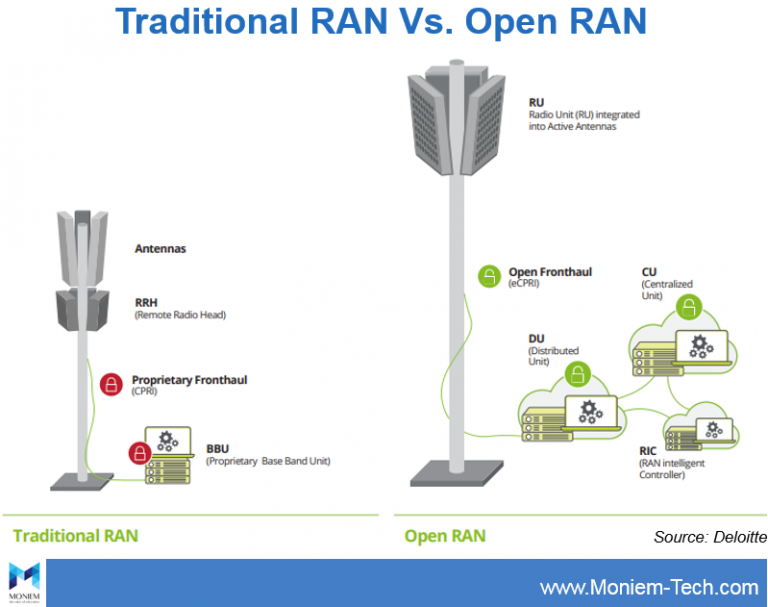
\includegraphics[width=0.8\textwidth]{assets/pics/bab3_10.png}
%     \caption{Perbandingan Traditional RAN vs O-RAN - Evolusi arsitektur menuju keterbukaan}
%     \label{fig:traditional_vs_oran}
% \end{figure}

Paradigma O-RAN berlandaskan pada tiga pilar utama yang mengubah landscape industri telekomunikasi. Openness dicapai melalui standardisasi interface yang memungkinkan komponen dari berbagai vendor bekerja secara seamless, mengurangi vendor lock-in yang selama ini menjadi tantangan operator jaringan. Intelligence terintegrasi melalui RAN Intelligent Controller yang memfasilitasi optimisasi real-time menggunakan machine learning dan AI untuk prediksi, otomasi, dan adaptasi dinamis terhadap kondisi jaringan yang berubah.

Virtualization memungkinkan disagregasi fungsi RAN tradisional menjadi komponen software yang dapat berjalan pada hardware commodity, sehingga menciptakan fleksibilitas deployment yang bagus. Pendekatan cloud-native ini memungkinkan scaling horizontal, resiliensi tinggi, dan tahap operasional yang lebih efisien melalui prinsip software-defined infrastructure.

\textbf{Ekosistem dan Competitive Landscape} O-RAN menciptakan marketplace teknologi yang memungkinkan vendor spesialis berkontribusi dalam segmen keahlian mereka tanpa harus menyediakan solusi end-to-end. Perubahan ini mendorong inovasi accelerated, competitive pricing, dan diversifikasi supplier chain yang meningkatkan resiliensi operasional.

Certification dan testing framework yang komprehensif memastikan interoperability tingkat tinggi antara komponen multi-vendor. O-RAN Alliance mengembangkan test specifications dan sertifikasi yang aktif untuk memvalidasi kompliansi terhadap standard O-RAN, manghasilkan confidence level yang tinggi dalam deployment production environments.

\subsection{Arsitektur dan Disagregasi Fungsional}

Arsitektur O-RAN mengimplementasikan functional split yang memisahkan base station tradisional menjadi entitas logis yang dapat di-deploy pada platform hardware berbeda-beda. Pendekatan ini memungkinkan optimisasi placement berdasarkan kebutuhan latency, transport network capabilities, dan konsiderasi ekonomi.

% \begin{figure}[htbp]
%     \centering
%     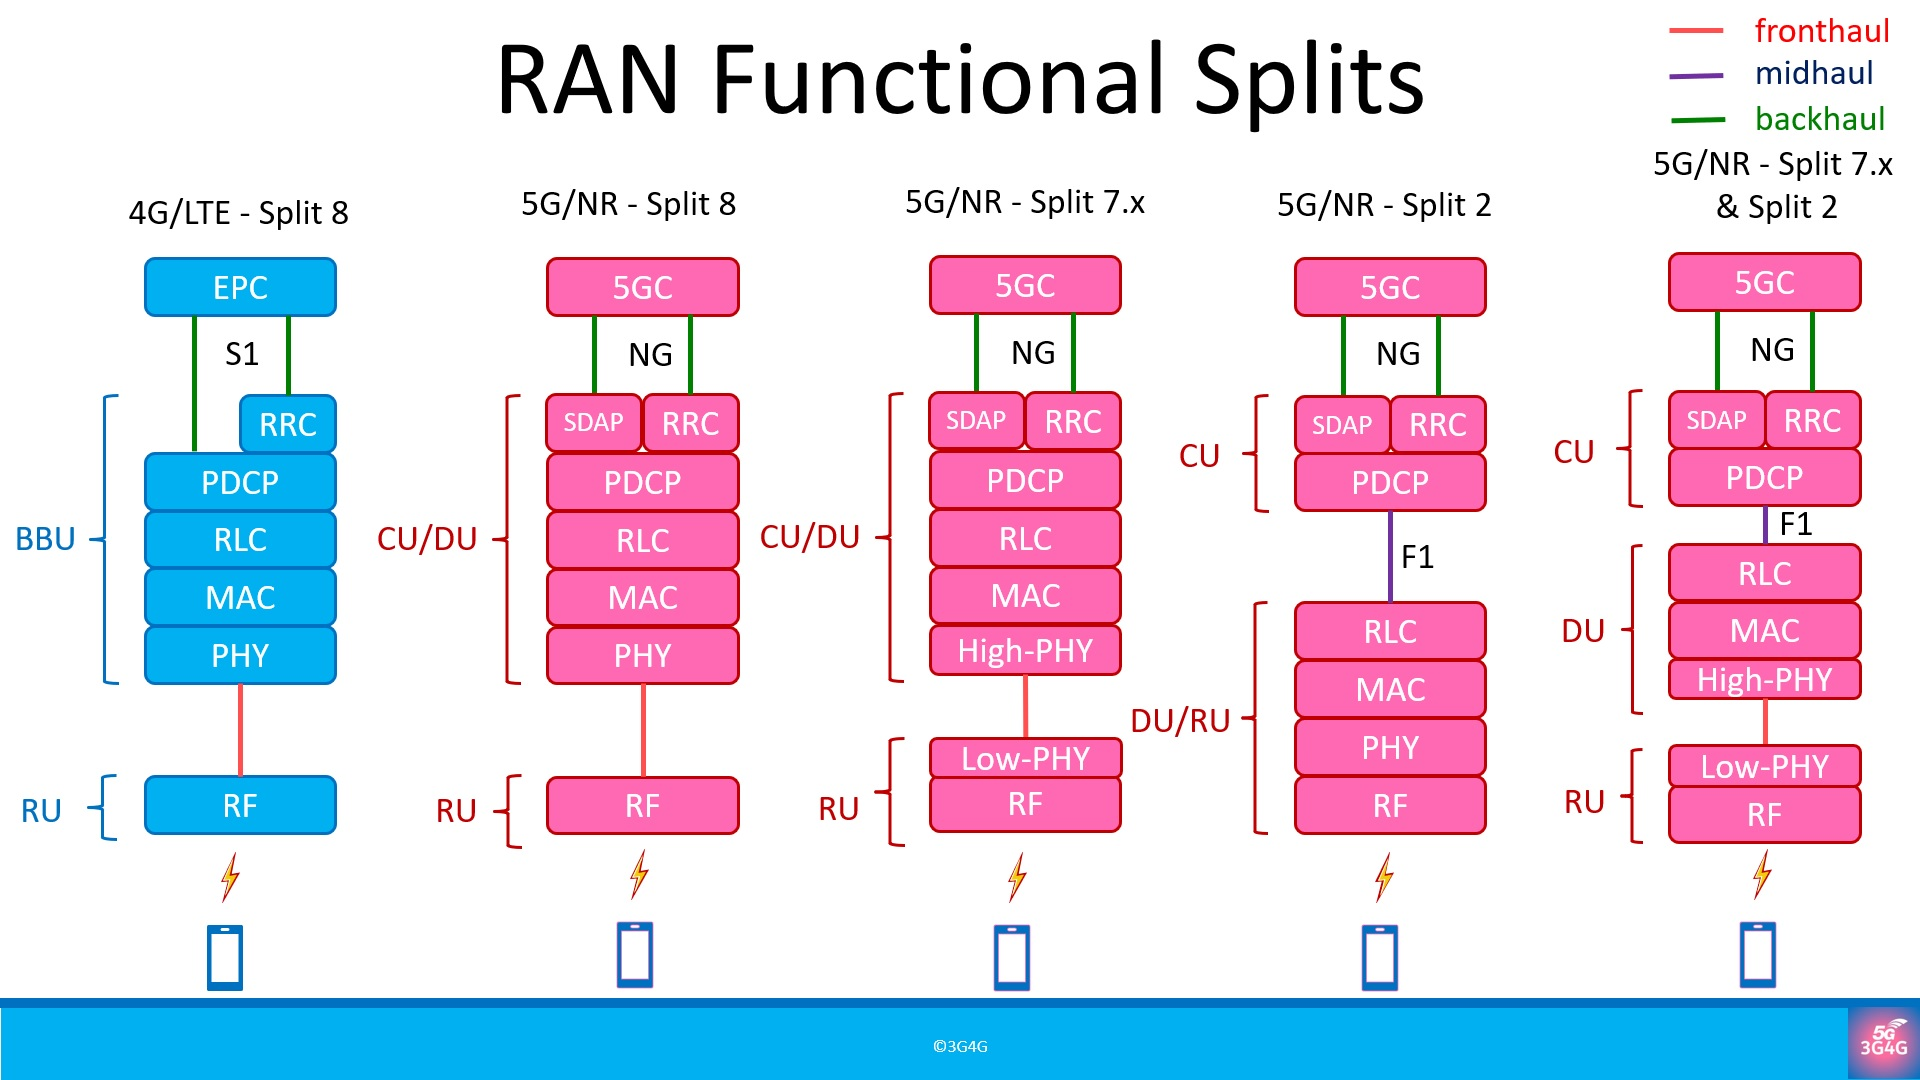
\includegraphics[width=0.8\textwidth]{assets/pics/bab3_11.png}
%     \caption{Arsitektur O-RAN - Disagregasi fungsional dan komponen utama}
%     \label{fig:oran_architecture}
% \end{figure}

\textbf{Radio Unit (O-RU)} menangani radio frequency processing dan antenna interface, beroperasi pada lapisan fisik terendah dengan batasan real-time yang ketat. O-RU dapat berupa dedicated hardware atau software-defined radio yang mendukung banyak frequency bands dan beamforming capabilities. Positioning O-RU umumnya co-located dengan antenna systems untuk meminimalkan RF losses dan mempertahankan signal integrity.

\textbf{Distributed Unit (O-DU)} mengimplementasikan real-time Layer 1 dan Layer 2 protocol processing dengan timing requirements yang kritis untuk operasi radio yang proper. O-DU dapat di-deploy sebagai alat terdedikasi di situs base station atau sebagai virtualized functions dalam fasilitas edge computing, tergantung pada transport latency dan processing requirements.

\textbf{Centralized Unit (O-CU)} mengelola higher-layer functions termasuk Radio Resource Control (RRC), Packet Data Convergence Protocol (PDCP), dan Service Data Adaptation Protocol (SDAP). O-CU dapat di-centralize untuk melayani multiple O-DU, memungkinkan coordination functions seperti carrier aggregation, dual connectivity, dan inter-cell interference mitigation yang lebih efektif.

\textbf{RAN Intelligent Controller Architecture} terdiri dari dua komponen complementary yang beroperasi pada skala waktu berbeda. Near Real-Time RIC beroperasi dengan response time 10ms hingga 1 detik untuk optimisasi kecepatan, sementara Non Real-Time RIC menangani policy management dan analytics pada time scale yang lebih panjang.

Near-RT RIC meng-host xApps yang mengimplementasikan control algorithms spesifik seperti traffic steering, load balancing, quality of experience optimization, dan interference mitigation. Multi-vendor xApp ecosystem memungkinkan specialized vendors berkontribusi algorithmic innovations tanpa perlu deep integration dengan RAN infrastructure.

Non-RT RIC mengelola kebijakan secara network-wide, trend analysis, dan long-term optimization. rApps dalam Non-RT RIC menganalisis historical data, network performance, dan objektif-objektif lainnya untuk menghasilkan kebijakan yang kemudian di-translate menjadi action controls oleh Near-RT RIC.

\subsection{Interface Standardisasi O-RAN}

Ekosistem O-RAN didefinisikan oleh sebuah set interfaces terstandarisasi yang memungkinkan interoperability antara komponen vendor berbeda. Setiap interface memiliki requirement spesifik untuk memastikan perilaku yang konsisten pada kasus multi-vendor deployment.

% \begin{figure}[htbp]
%     \centering
%     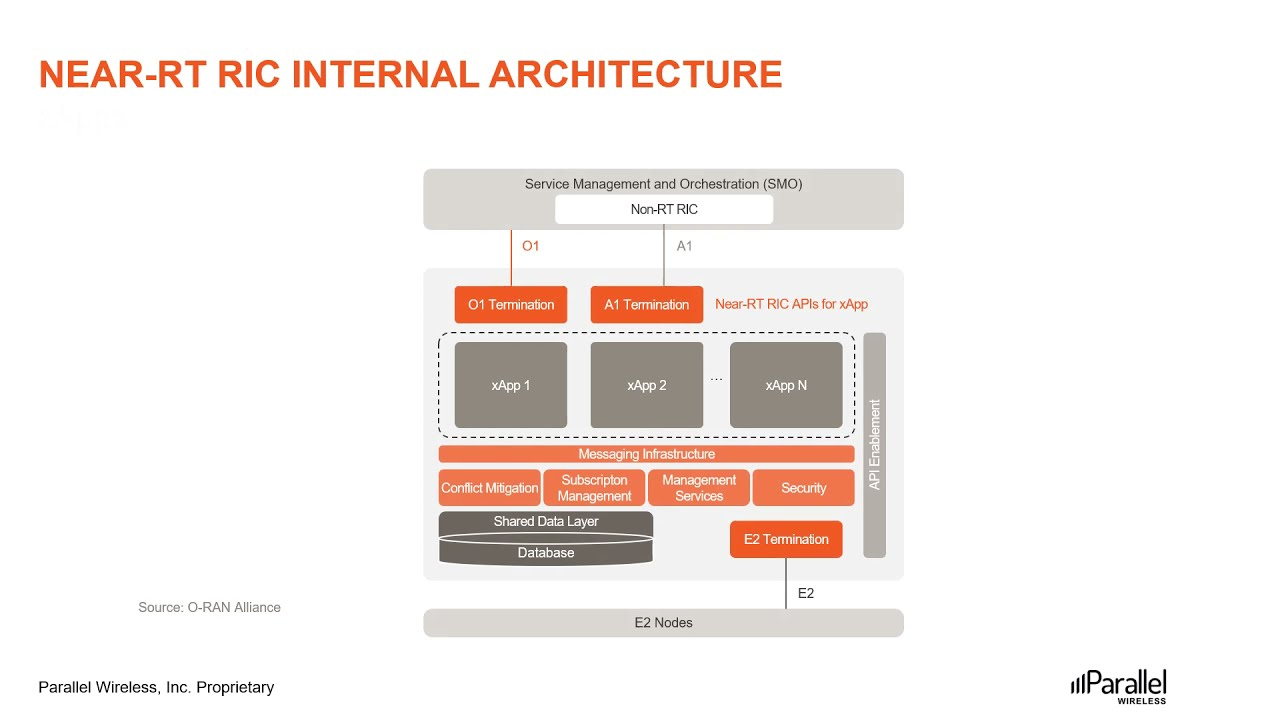
\includegraphics[width=0.8\textwidth]{assets/pics/bab3_12.png}
%     \caption{Interface O-RAN - Konektivitas antar komponen sistem}
%     \label{fig:oran_interfaces}
% \end{figure}

\textbf{Open Fronthaul Interface} menghubungkan O-RU dengan O-DU dan merepresentasikan salah satu interface paling kritis dalam arsitektur O-RAN. Interface ini menghandle transport digital radio samples, kontrol informasi, dan sinkronisasi data dengan stringent latency dan kebutuhan bandwidth.

Enhanced Common Public Radio Interface (eCPRI) dan Radio over Ethernet protocols menyediakan mekanisme transport yang efisien dengan algoritma kompresi efisien untuk optimisasi bandwidth. Precision Time Protocol (PTP) memastikan sinkronisasi yang akurat antara O-RU dan O-DU yang sangat penting untuk operasi radio yang benar, terutama dalam coordinated multi-point transmissions dan carrier aggregation.

\textbf{F1 Interface Connectivity} menghubungkan O-DU dengan O-CU menggunakan 3GPP standardized protocols. F1-Control Plane menangani signaling dan manajemen pesan yang dikirim dengan jaminan reliabilitas, sementara F1-User Plane meng-forward user traffic dengan pemisahan QoS dan traffic handling yang sesuai.

F1 interface mendukung skenario deployment variatif, termasuk centralized O-CU yang menyediakan banyak O-DU, distributed O-CU deployments untuk aplikasi yang sensitif waktu, dan integrasi dengan teknologi transport network berbeda dari fiber hingga microwave backhaul.

\textbf{A1 Policy Interface} memfasilitasi komunikasi antara Non-RT RIC dan Near-RT RIC untuk distribusi kebijakan dan intent propagation. Interface A1 memungkinkan Non-RT RIC mengonfigurasi Near-RT RIC dengan kebijakan high-level yang kemudian diinterpret dan dijalankan oleh xApps dalam bentuk tindakan kontrol spesifik.

Kerangka kebijakan ini mendukung beragam jenis kebijakan termasuk kebijakan alokasi sumber daya, aturan policy QoS, dan objektif optimisasi jaringan yang dapat disesuaikan dengan kondisi jaringan spesifik dan kebutuhan bisnis.

\textbf{Control Interface E2} menghubungkan Near-RT RIC dengan elemen jaringan O-RAN untuk kontrol dan monitoring waktu nyata. E2-Control Plane menangani pertukaran pesan kontrol dengan pengiriman terjamin, sementara E2-User Plane memungkinkan pengarahan lalu lintas dan modifikasi user plane.

Konsep Model Layanan menyediakan pola interaksi terstandarisasi antara RIC dan berbagai jenis elemen jaringan, dengan fleksibilitas untuk ekstensi spesifik vendor dan kustomisasi yang mempertahankan prinsip interoperabilitas.

\subsection{Manajemen Layanan dan Orkestrasi}

Kerangka Manajemen Layanan dan Orkestrasi dalam O-RAN menyediakan kemampuan manajemen komprehensif untuk pengelolaan siklus hidup komponen O-RAN, penegakan kebijakan, dan integrasi dengan ekosistem manajemen jaringan yang lebih luas.

\textbf{Manajemen Siklus Hidup Otomatis} mencakup penyebaran, konfigurasi, monitoring, dan pemeliharaan fungsi O-RAN di seluruh infrastruktur terdistribusi. SMO terintegrasi dengan platform cloud orchestration untuk penyediaan sumber daya otomatis dan penyebaran fungsi jaringan berdasarkan permintaan layanan dan requirements kinerja.

Model penyebaran berbasis kontainer memfasilitasi penskalaan cepat dan migrasi fungsi untuk optimisasi pemanfaatan sumber daya dan peningkatan kinerja. Integrasi DevOps mendukung jalur integrasi berkelanjutan/penyebaran berkelanjutan untuk pembaruan perangkat lunak otomatis, peluncuran fitur, dan manajemen konfigurasi di seluruh penyebaran skala besar.

\textbf{Manajemen dan Penegakan Kebijakan} memungkinkan definisi kebijakan terpusat dan penegakan konsisten di seluruh ekosistem O-RAN. Cakupan kebijakan mencakup aturan alokasi sumber daya, persyaratan keamanan, objektif kinerja, dan batasan kepatuhan yang secara otomatis ditegakkan melalui sistem otomatis.

Kemampuan jaringan intent based memungkinkan objektif bisnis tingkat tinggi diterjemahkan menjadi konfigurasi dan behavior jaringan spesifik melalui machine learning dan algoritma AI yang memahami hubungan antara maksud bisnis high-level dan implementasi teknis.

\textbf{Integrasi dan Konektivitas Ekosistem} SMO menyediakan interface terstandarisasi untuk integrasi dengan sistem OSS/BSS yang ada, platform monitoring jaringan, dan alat manajemen third party. API dan model data memfasilitasi pertukaran informasi yang mulus dan tindakan manajemen terkoordinasi di seluruh lingkungan multi-vendor.

Kemampuan fault correlation dan analisis akar masalah menggabungkan informasi dari berbagai komponen O-RAN untuk menyediakan visibilitas kesehatan jaringan komprehensif dan tindakan perbaikan otomatis untuk skenario kegagalan umum. Analitik lanjutan memungkinkan pemeliharaan prediktif dan resolusi masalah proaktif sebelum dampak pada layanan dan pengguna terjadi.

%-----------------------------------------------------------------------------%
\section{O1 Interface} 
%-----------------------------------------------------------------------------%

\subsection{Gambaran Umum O1 Interface}

Interface O1 merupakan komponen kritis dalam arsitektur O-RAN yang menyediakan kemampuan manajemen standar untuk elemen jaringan O-RAN. Interface ini memungkinkan Service Management and Orchestration (SMO) framework untuk melakukan konfigurasi, monitoring, dan kontrol terhadap berbagai komponen O-RAN seperti O-CU, O-DU, dan Near-RT RIC.

% \begin{figure}[h]
%     \centering
%     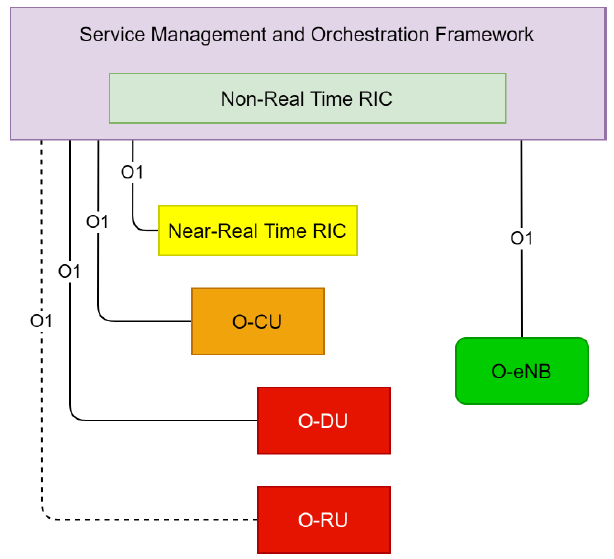
\includegraphics[width=0.8\textwidth]{assets/pics/bab3_14.png}
%     \caption{Arsitektur O1 Interface}
%     \label{fig:o1_interface}
% \end{figure}

O1 interface mengadopsi protokol NETCONF (Network Configuration Protocol) sebagai mekanisme transport utama, dengan model data yang didefinisikan menggunakan YANG (Yet Another Next Generation) untuk memastikan interoperabilitas dan standarisasi dalam manajemen jaringan. Pendekatan ini memungkinkan manajemen terpusat yang konsisten dan dapat diandalkan di seluruh ekosistem O-RAN multi-vendor.

\subsection{Protokol NETCONF}

NETCONF merupakan protokol manajemen jaringan yang dirancang untuk menyediakan mekanisme sederhana namun powerful untuk menginstal, memanipulasi, dan menghapus konfigurasi perangkat jaringan. Protokol ini menggunakan paradigma Remote Procedure Call (RPC) dengan encoding XML untuk komunikasi antara klien manajemen dan server yang dikelola.

% \begin{figure}[h]
%     \centering
%     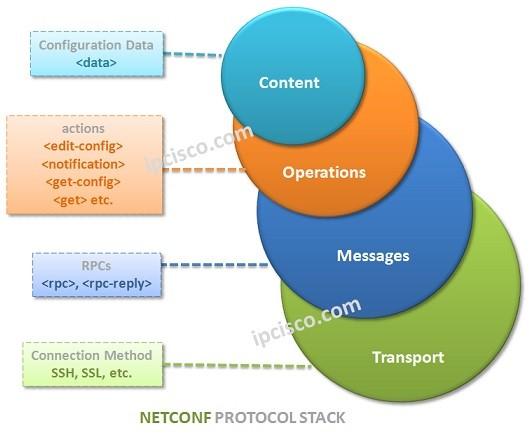
\includegraphics[width=0.8\textwidth]{assets/pics/bab3_15.png}
%     \caption{Struktur Protokol NETCONF}
%     \label{fig:netconf_structure}
% \end{figure}

Operasi dasar NETCONF mencakup get-config untuk mengambil konfigurasi perangkat, edit-config untuk memodifikasi konfigurasi, copy-config untuk menyalin konfigurasi antar datastore, dan delete-config untuk menghapus konfigurasi. Setiap operasi dilakukan dalam konteks datastore yang berbeda seperti running, candidate, dan startup configuration.

Model data YANG menyediakan bahasa pemodelan yang kuat untuk mendefinisikan struktur data, batasan, dan hubungan dalam konfigurasi jaringan. YANG memungkinkan definisi yang tepat tentang elemen konfigurasi, tipe data, validasi, dan semantik operasional yang dapat dipahami secara konsisten oleh implementasi yang berbeda.

Manajemen sesi dalam NETCONF memungkinkan multiple klien untuk berinteraksi dengan perangkat yang sama secara bersamaan dengan mekanisme locking dan koordinasi untuk mencegah konflik konfigurasi. Capability discovery memungkinkan klien untuk menentukan fitur dan model data yang didukung oleh server target.

\subsection{Performance Management melalui O1}

Manajemen kinerja melalui interface O1 menyediakan kemampuan komprehensif untuk mengumpulkan, menganalisis, dan melaporkan metrik kinerja dari elemen jaringan O-RAN. Sistem ini memungkinkan monitoring waktu nyata dan analisis historis untuk optimisasi jaringan dan deteksi masalah.

Pengumpulan pengukuran kinerja dilakukan melalui mekanisme subscription-based dimana SMO dapat berlangganan metrik kinerja spesifik dari elemen jaringan dengan interval pengumpulan yang dapat dikonfigurasi. Model data YANG mendefinisikan struktur Key Performance Indicators (KPI) yang terstandarisasi untuk memastikan konsistensi interpretasi metrik di seluruh vendor.

KPI utama yang dipantau mencakup throughput cell, jumlah pengguna aktif, utilisasi sumber daya radio, tingkat kesalahan block, latensi user plane, dan metrik kualitas layanan aplikasi. Agregasi dan korelasi metrik dari multiple elemen jaringan memberikan pandangan holistik tentang kinerja jaringan end-to-end.

Sistem pelaporan dan alerting terintegrasi memungkinkan deteksi otomatis kondisi abnormal dan notifikasi proaktif kepada operator jaringan. Threshold-based monitoring dan trend analysis membantu mengidentifikasi degradasi kinerja sebelum berdampak pada pengalaman pengguna.

\subsection{Configuration Management melalui O1}

Manajemen konfigurasi melalui interface O1 menyediakan framework terstandarisasi untuk mengelola parameter operasional dan kebijakan elemen jaringan O-RAN. Sistem ini mendukung konfigurasi terpusat dengan kemampuan validasi, konsistensi, dan rollback yang robust.

Model data konfigurasi didefinisikan menggunakan YANG untuk memastikan struktur yang konsisten dan interpretasi parameter yang seragam di seluruh implementasi vendor. Hierarki konfigurasi mengorganisir parameter berdasarkan domain fungsional seperti radio resource management, mobility management, dan quality of service.

Operasi konfigurasi mendukung atomic transactions dimana perubahan multiple dapat dikelompokkan dan diimplementasikan secara bersamaan untuk mempertahankan konsistensi sistem. Validasi semantic memastikan bahwa konfigurasi yang diusulkan adalah valid dan tidak akan menyebabkan konflik operasional.

Mekanisme rollback memungkinkan pemulihan cepat dari perubahan konfigurasi yang bermasalah dengan menyimpan snapshot konfigurasi sebelumnya. Version control dan audit trail menyediakan visibilitas historis terhadap perubahan konfigurasi untuk compliance dan troubleshooting.

%-----------------------------------------------------------------------------%
\section{Virtual Event Streaming (VES)}
%-----------------------------------------------------------------------------%

\subsection{Gambaran Umum VES}

Virtual Event Streaming (VES) merupakan spesifikasi standar industri yang mendefinisikan format dan protokol untuk streaming event data dari fungsi jaringan virtual dan elemen jaringan fisik ke sistem manajemen dan analitik. VES memungkinkan arsitektur event-driven yang mendukung monitoring waktu nyata, analitik, dan otomasi dalam lingkungan jaringan modern.

Arsitektur event-driven yang didukung VES memberikan kemampuan untuk merespons kondisi jaringan secara real-time dengan mengirimkan event yang terstruktur dan terstandarisasi ke sistem pengumpul dan analisis. Pendekatan ini memungkinkan deteksi masalah yang cepat, optimisasi proaktif, dan otomasi respons berdasarkan kondisi operasional yang berubah.

Streaming data waktu nyata melalui VES mendukung use case seperti fault management, performance monitoring, security event correlation, dan capacity planning dengan memberikan visibilitas mendalam terhadap operasi jaringan dan perilaku aplikasi.

% \begin{figure}[h]
%     \centering
%     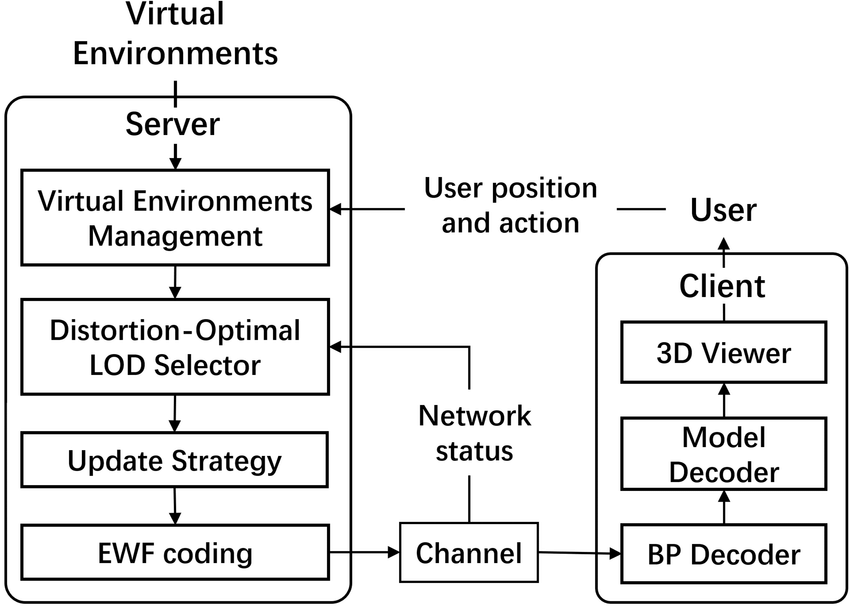
\includegraphics[width=0.8\textwidth]{assets/pics/bab3_16.png}
%     \caption{Arsitektur VES}
%     \label{fig:ves_architecture}
% \end{figure}

\subsection{Model Event VES}

Struktur event VES didefinisikan dengan skema JSON lengkap yang mencakup header umum dan domain-specific fields. Header event berisi metadata seperti timestamp, source identifier, event type, dan correlation information yang memungkinkan identifikasi dan pemrosesan event yang akurat.

Domain event dikategorikan berdasarkan jenis informasi yang dibawa seperti fault events, performance measurement events, syslog events, threshold crossing alerts, dan heartbeat events. Setiap kategori memiliki struktur data spesifik yang dioptimalkan untuk jenis informasi yang ditransmisikan.

Siklus hidup event mencakup generasi event di source, transmisi melalui jaringan, pengumpulan di collector, dan pemrosesan di sistem analitik. Event correlation memungkinkan hubungan antara event yang terkait untuk analisis root cause dan impact assessment yang lebih akurat.

Format data dan skema JSON menyediakan struktur yang fleksibel namun terstandarisasi untuk representasi event dengan dukungan untuk extensibility dan vendor-specific fields dalam kerangka kerja yang terdefinisi dengan baik.

\subsection{VES dalam Lingkungan Telco}

Integrasi VES dalam lingkungan telekomunikasi memungkinkan pengumpulan event komprehensif dari berbagai fungsi jaringan termasuk Virtual Network Functions (VNF), Container Network Functions (CNF), dan Physical Network Functions (PNF). Standardisasi format event memfasilitasi interoperabilitas multi-vendor dan analisis terpusat.

Event pengukuran kinerja melalui VES menyediakan streaming metrik kinerja real-time seperti throughput, latency, error rates, dan resource utilization dari berbagai komponen jaringan. Agregasi dan korelasi metrik ini memberikan insight holistik tentang kesehatan dan kinerja jaringan end-to-end.

Event notifikasi fault menyediakan informasi real-time tentang kegagalan komponen, degradasi kinerja, dan kondisi abnormal dalam jaringan. Sistem event correlation dapat mengidentifikasi pola fault dan memberikan automated remediation actions untuk mempercepat resolusi masalah.

Sistem monitoring dan analitik dapat mengintegrasikan VES events dengan platform big data dan machine learning untuk predictive analytics, anomaly detection, dan optimization recommendations berdasarkan historical patterns dan real-time conditions.

%-----------------------------------------------------------------------------%
\section{Network Simulator 3 (NS-3)}
%-----------------------------------------------------------------------------%

\subsection{Gambaran Umum NS-3}

Network Simulator 3 (NS-3) merupakan simulator jaringan berbasis discrete-event yang dirancang khusus untuk keperluan penelitian dan pendidikan dalam bidang jaringan komputer. NS-3 menyediakan platform simulasi yang komprehensif untuk memodelkan berbagai teknologi jaringan, protokol, dan aplikasi dalam lingkungan yang dapat dikontrol dan direproduksi dengan akurat.

Karakteristik utama NS-3 sebagai simulator discrete-event memungkinkan pemodelan yang akurat dari perilaku jaringan dengan memproses kejadian dalam urutan waktu yang tepat. Simulator ini mendukung berbagai model jaringan mulai dari jaringan kabel tradisional hingga teknologi nirkabel modern seperti WiFi, LTE, dan 5G.

Dibandingkan dengan simulator jaringan lainnya, NS-3 menyediakan model yang lebih detail dan akurat dengan dukungan untuk implementasi protokol dunia nyata dan integrasi dengan network stack yang sesungguhnya. Fleksibilitas dan kemampuan perluasan NS-3 memungkinkan peneliti untuk mengembangkan model khusus dan mengintegrasikan teknologi jaringan yang baru.

% \begin{figure}[h]
%     \centering
%     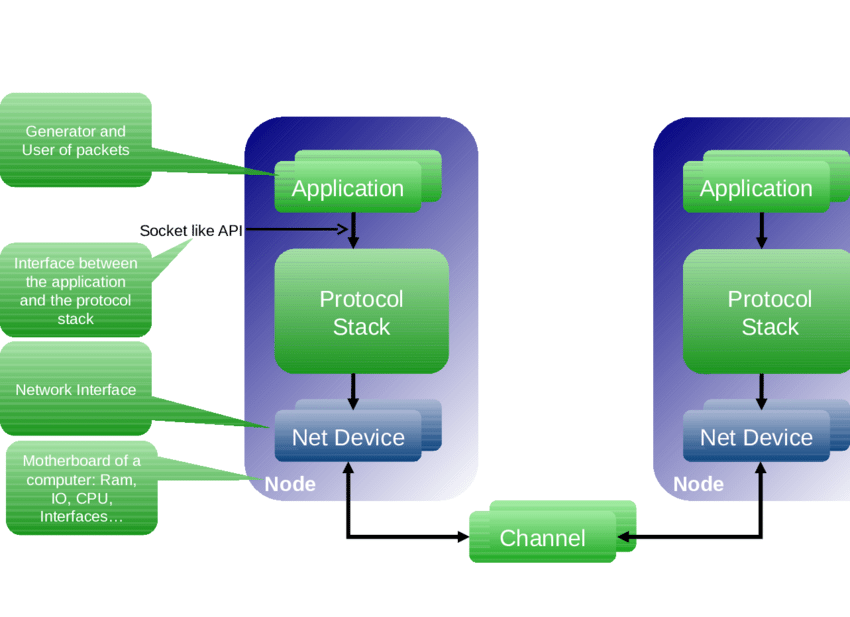
\includegraphics[width=0.8\textwidth]{assets/pics/bab3_17.png}
%     \caption{NS-3 General Architecture}
%     \label{fig:ns3_architecture}
% \end{figure}

\subsection{Arsitektur NS-3}

Mesin simulasi inti NS-3 dibangun dengan arsitektur modular yang memisahkan kernel simulasi dari model jaringan spesifik. Penjadwal kejadian mengelola eksekusi event berdasarkan waktu simulasi dengan dukungan untuk berbagai algoritma penjadwalan yang dapat disesuaikan dengan kebutuhan simulasi tertentu.

Model jaringan dan protokol dalam NS-3 diorganisir dalam hierarki yang mencerminkan arsitektur jaringan nyata dari lapisan fisik hingga lapisan aplikasi. Setiap lapisan memiliki model yang dapat dikonfigurasi dan diperluas untuk mengakomodasi berbagai teknologi dan protokol jaringan yang berbeda.

Simulasi lapisan aplikasi mendukung berbagai jenis aplikasi jaringan seperti transfer data massal, generator lalu lintas on-off, streaming video, dan aplikasi waktu nyata. Model aplikasi dapat disesuaikan untuk mensimulasikan pola lalu lintas yang realistis dan menganalisis karakteristik kinerja yang spesifik.

Model mobilitas dalam NS-3 memungkinkan simulasi pergerakan node dalam jaringan nirkabel dengan berbagai pola mobilitas seperti random walk, kecepatan konstan, dan mobilitas berbasis jejak. Integrasi dengan model propagasi menyediakan simulasi yang akurat dari karakteristik kanal nirkabel dalam berbagai kondisi lingkungan.

\subsection{Simulasi WiFi dalam NS-3}

Implementasi model WiFi dalam NS-3 menyediakan dukungan komprehensif untuk berbagai standar IEEE 802.11 dengan detail implementasi yang akurat dari operasi lapisan MAC dan lapisan fisik. Model ini mendukung berbagai mode operasi termasuk mode infrastruktur dengan access point dan jaringan ad-hoc.

Model kanal dan propagasi dalam simulasi WiFi mencakup berbagai model path loss, model fading, dan pemodelan interferensi untuk mensimulasikan kondisi RF yang realistis. Penundaan propagasi, pelemahan sinyal, dan efek multipath dapat dimodelkan dengan akurasi tinggi untuk berbagai lingkungan penerapan.

Generasi lalu lintas dan analisis kinerja memungkinkan evaluasi komprehensif dari kinerja jaringan Wi-Fi dengan berbagai metrik seperti throughput, latensi, rasio pengiriman paket, dan konsumsi energi. Generator lalu lintas dapat dikonfigurasi untuk mensimulasikan berbagai skenario aplikasi dan pola perilaku pengguna.

Evaluasi kinerja dapat dilakukan dengan mengintegrasikan berbagai metrik dan analisis statistik untuk mengidentifikasi kemacetan, mengoptimalkan parameter jaringan, dan membandingkan berbagai skenario konfigurasi dalam lingkungan simulasi yang terkontrol.

% \begin{figure}[h]
%     \centering
%     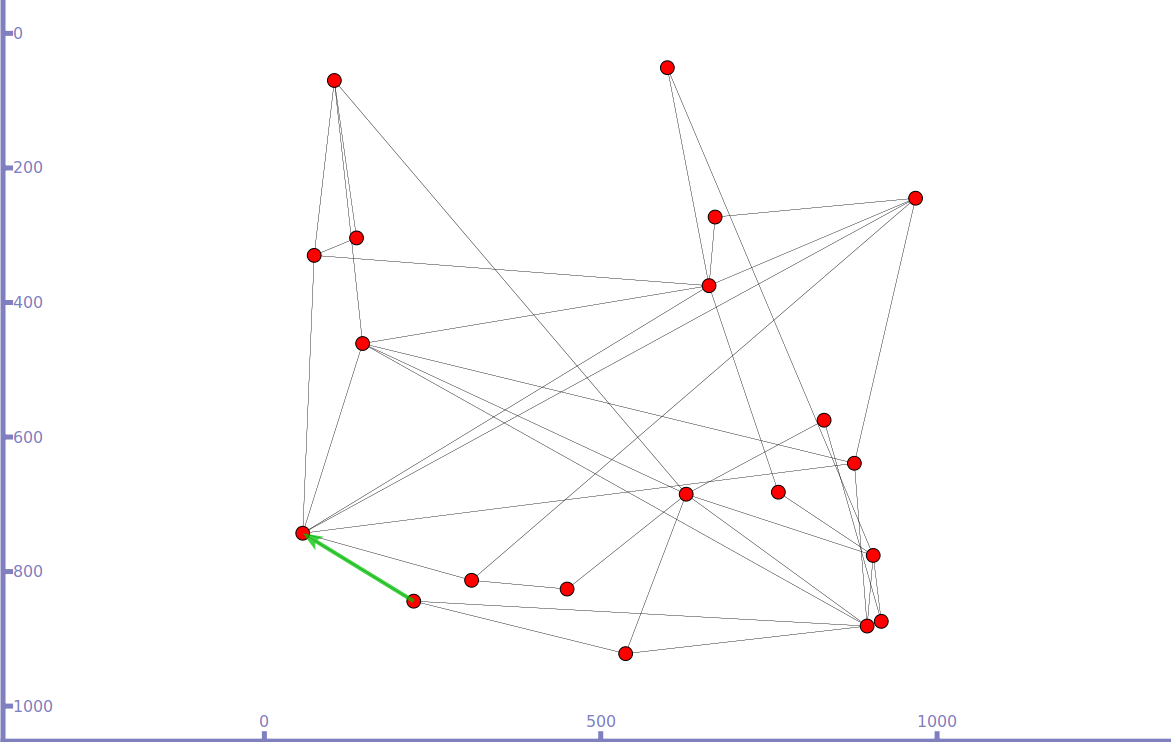
\includegraphics[width=0.8\textwidth]{assets/pics/bab3_18.png}
%     \caption{NS-3 WiFi Network Simulation}
%     \label{fig:ns3_wifi_simulation}
% \end{figure}

%-----------------------------------------------------------------------------%
\section{Manajemen dan Visualisasi Data}
%-----------------------------------------------------------------------------%

\subsection{InfluxDB}

InfluxDB merupakan basis data time-series yang dirancang khusus untuk menangani data yang memiliki komponen waktu sebagai dimensi utama. Konsep basis data time-series sangat relevan untuk aplikasi monitoring jaringan dimana metrik kinerja, log event, dan data pengukuran dikumpulkan secara berkelanjutan dengan cap waktu yang akurat.

Arsitektur InfluxDB dioptimalkan untuk penyerapan dan kueri data time-series berkinerja tinggi dengan dukungan untuk kompresi data otomatis, kebijakan retensi, dan kueri berkelanjutan. Mesin penyimpanan yang khusus memungkinkan penyimpanan dan pengambilan data yang efisien dengan volume tinggi dan pola kueri yang khas untuk beban kerja time-series.

Proses penyerapan data dalam InfluxDB mendukung berbagai protokol masukan termasuk HTTP API, UDP, dan integrasi dengan agen pengumpul seperti Telegraf. Penyerapan batch dan streaming waktu nyata memungkinkan fleksibilitas dalam strategi pengumpulan data berdasarkan kebutuhan aplikasi dan batasan infrastruktur.

Kemampuan kueri menggunakan InfluxQL (bahasa kueri mirip SQL) atau Flux (bahasa kueri fungsional) memberikan kemampuan analitik yang kuat untuk analisis data time-series, agregasi, dan transformasi. Fungsi bawaan untuk analisis statistik, rata-rata bergerak, dan deteksi tren memfasilitasi analitik lanjutan pada data monitoring.

% \begin{figure}[htbp]
%     \centering
%     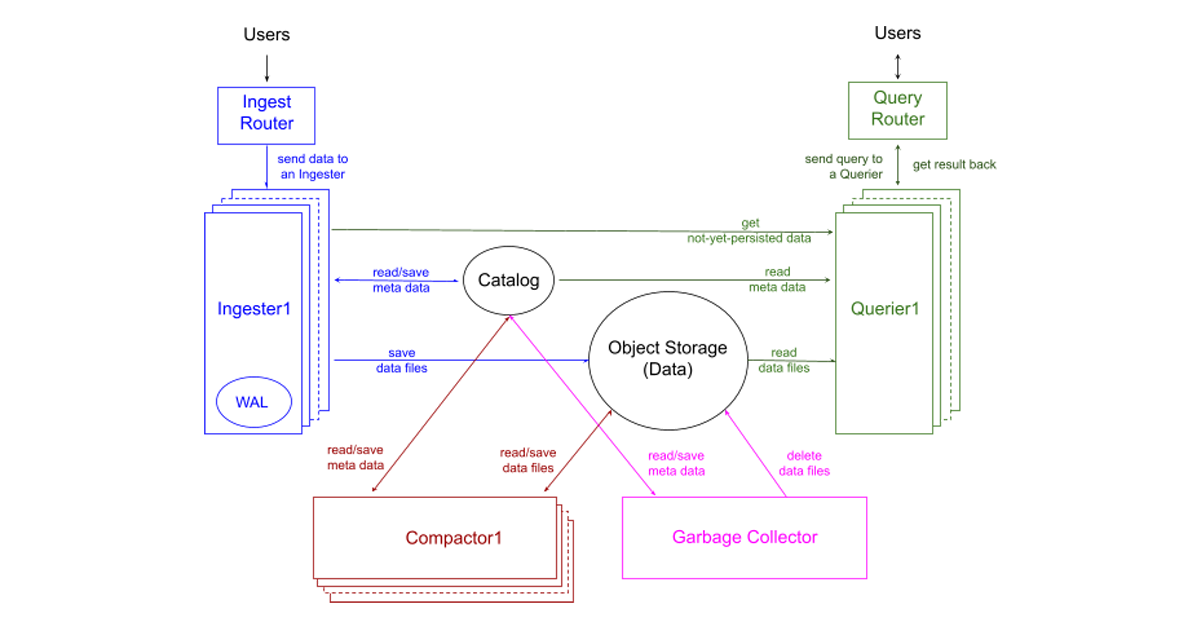
\includegraphics[width=0.8\textwidth]{assets/pics/bab3_19.png}
%     \caption{Arsitektur InfluxDB - Penyimpanan time-series teroptimasi}
%     \label{fig:influxdb_architecture}
% \end{figure}

\subsection{Grafana}

Grafana merupakan platform visualisasi data sumber terbuka yang menyediakan kemampuan untuk membuat dashboard interaktif dan informatif dari berbagai sumber data. Platform ini sangat powerful untuk aplikasi monitoring dengan dukungan untuk visualisasi data waktu nyata dan sistem peringatan.

Pembuatan dan manajemen dashboard dalam Grafana menggunakan interface berbasis web yang intuitif dengan komponen drag-and-drop, panel yang dapat dikonfigurasi, dan opsi visualisasi yang kaya. Dukungan template dan variabel memungkinkan pembuatan dashboard yang dinamis dan dapat digunakan kembali untuk berbagai lingkungan dan kasus penggunaan.

Monitoring waktu nyata didukung melalui kemampuan penyegaran otomatis, streaming data waktu nyata, dan visualisasi responsif yang memberikan wawasan langsung tentang kinerja sistem dan kesehatan jaringan. Integrasi dengan berbagai sumber data memungkinkan tampilan terpadu dari beberapa sistem monitoring.

Sistem peringatan dan notifikasi terintegrasi memungkinkan monitoring proaktif dengan peringatan berbasis ambang batas, deteksi anomali, dan pengiriman notifikasi multi-saluran melalui email, Slack, webhook, dan integrasi lainnya untuk respons insiden yang cepat.

% \begin{figure}[htbp]
%     \centering
%     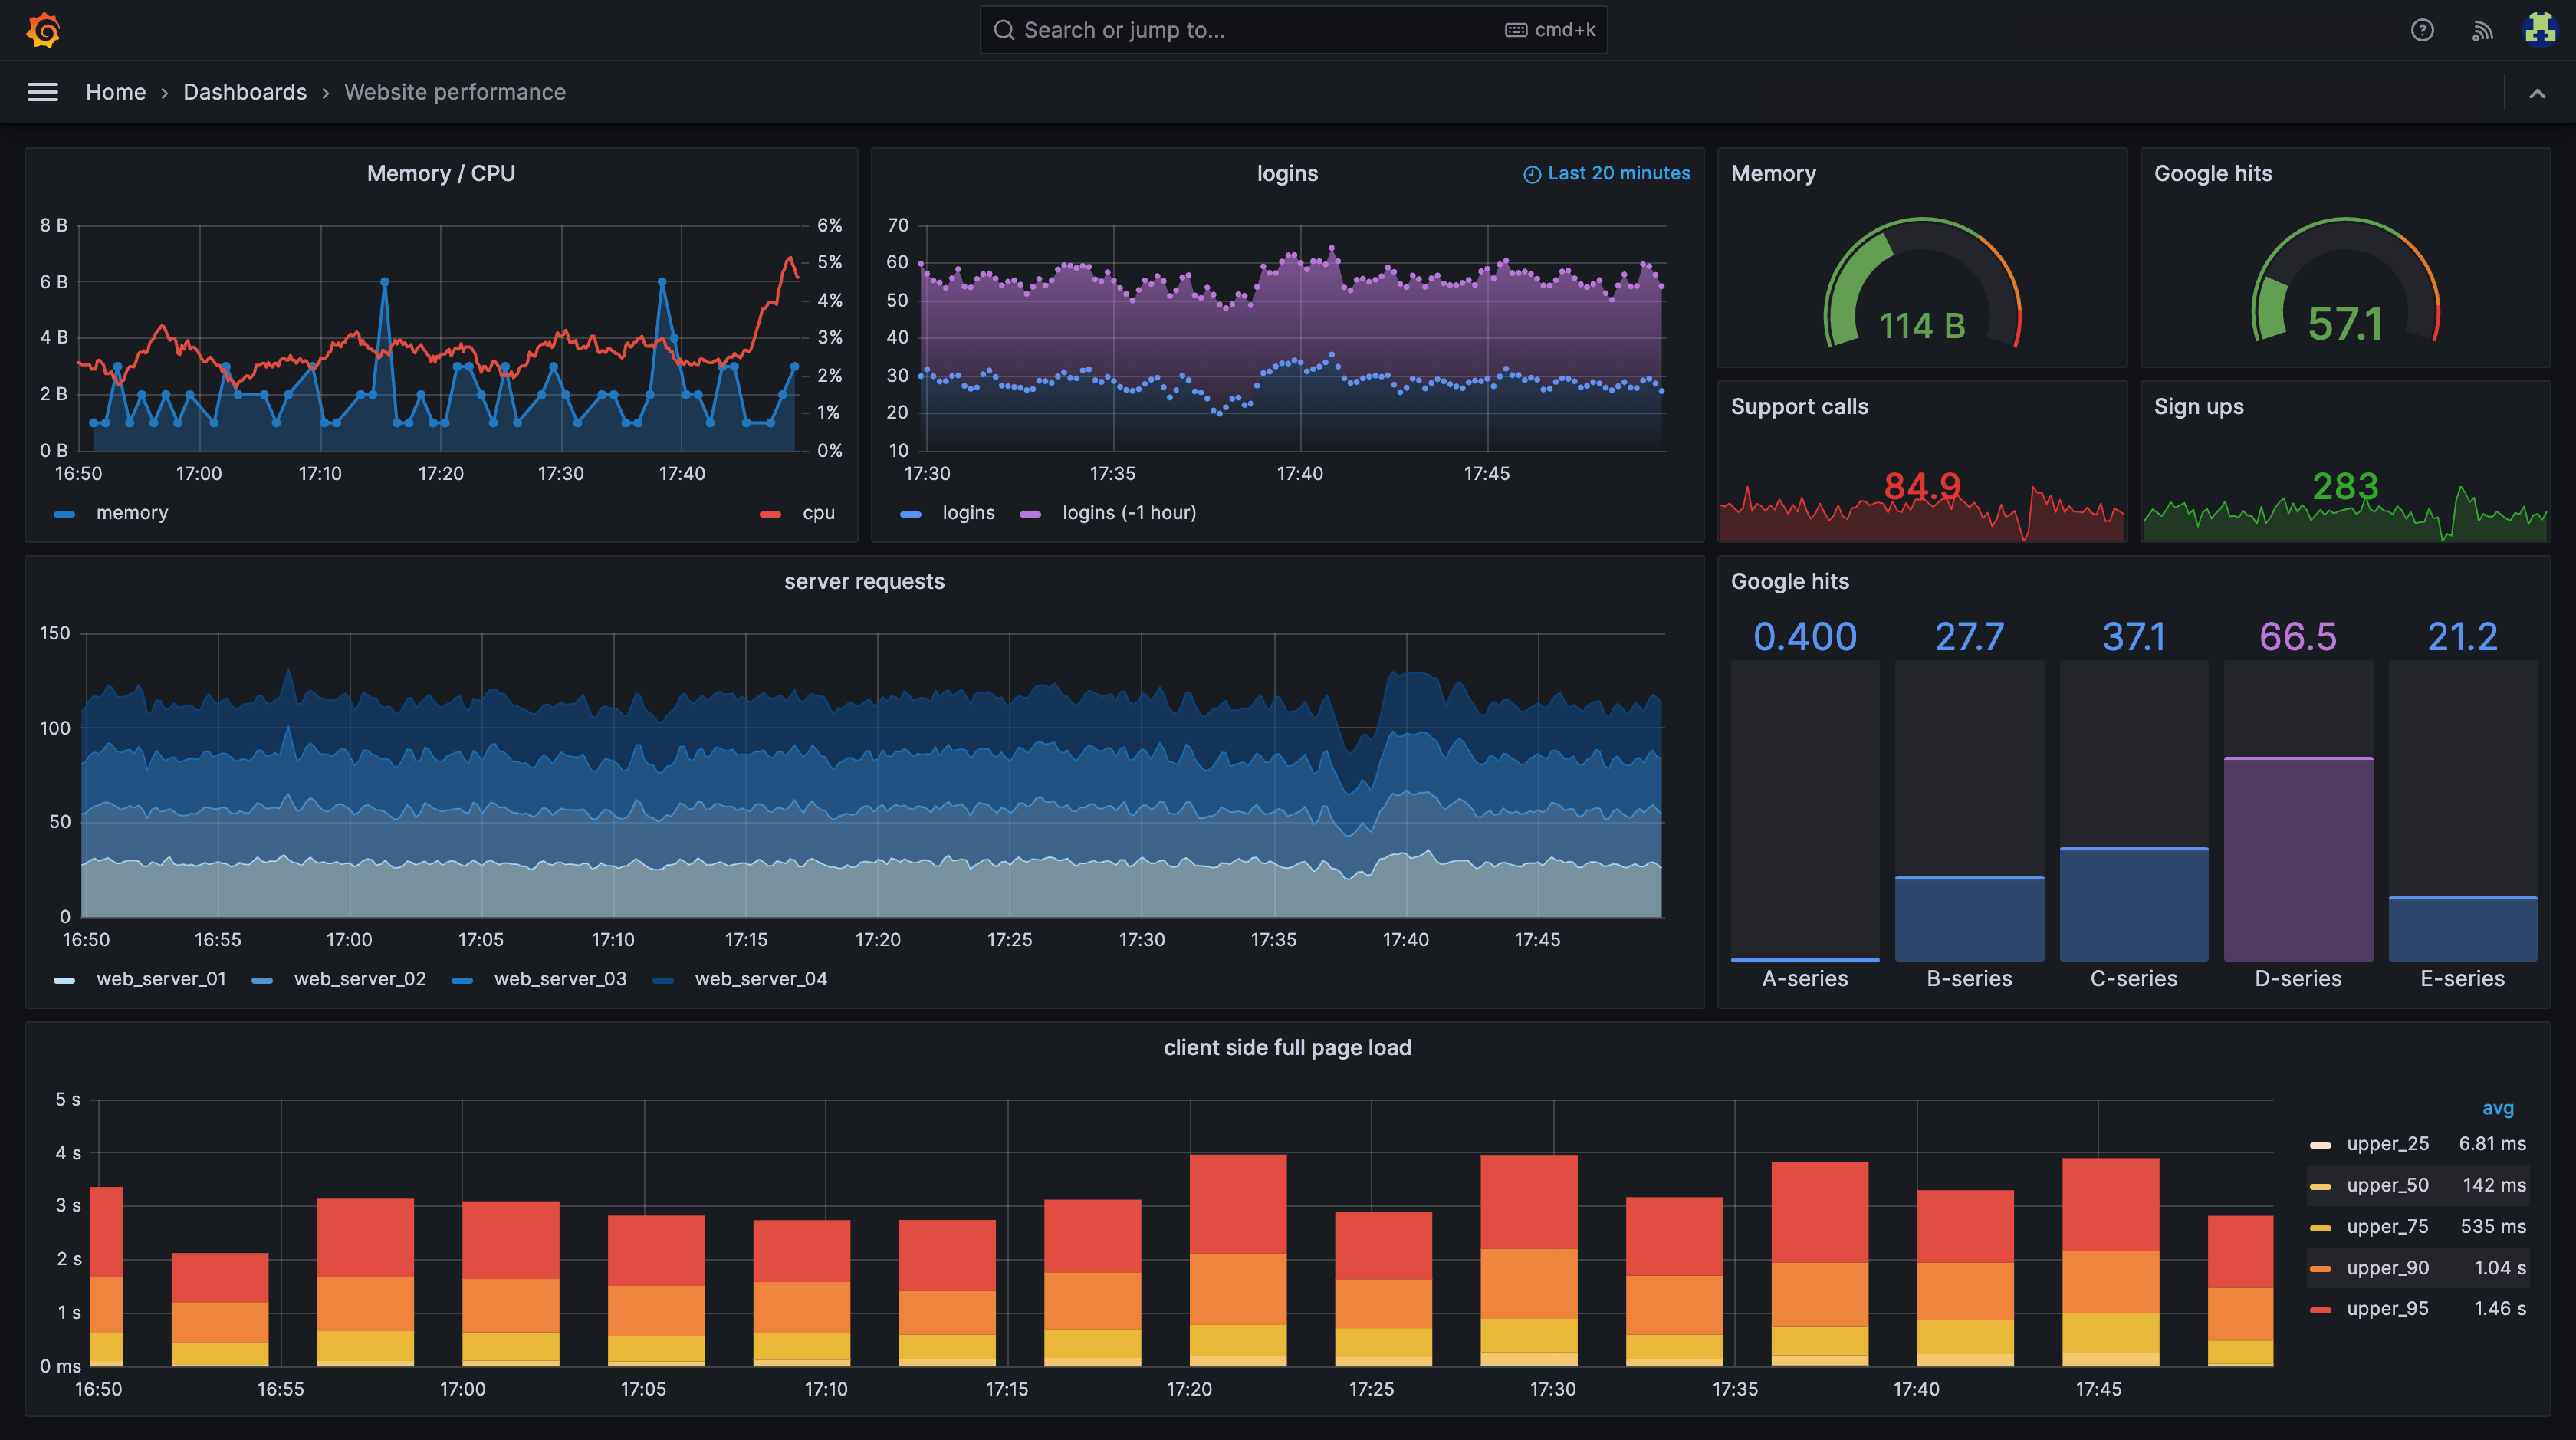
\includegraphics[width=0.8\textwidth]{assets/pics/bab3_20.png}
%     \caption{Arsitektur Grafana - Visualisasi data monitoring}
%     \label{fig:grafana_architecture}
% \end{figure}

\subsection{Integrasi InfluxDB-Grafana}

Pengaturan pipeline data antara InfluxDB dan Grafana melibatkan konfigurasi koneksi sumber data, autentikasi, dan optimisasi kueri untuk memastikan kinerja yang optimal dalam pengambilan dan visualisasi data. Strategi connection pooling dan caching dapat diimplementasikan untuk skalabilitas yang lebih baik.

Praktik terbaik untuk visualisasi mencakup pemilihan jenis grafik yang sesuai untuk karakteristik data yang berbeda, skema warna yang informatif, pemilihan rentang waktu yang relevan, dan tingkat agregasi yang memberikan wawasan bermakna tanpa membebani pengguna dengan detail yang berlebihan.

Dashboard monitoring kinerja harus dirancang dengan mempertimbangkan pengalaman pengguna, waktu muat, dan pemanfaatan sumber daya. Pengorganisasian dashboard dalam folder, penggunaan tag dan anotasi, serta implementasi kontrol akses berbasis peran memfasilitasi manajemen dashboard yang efektif dalam lingkungan enterprise.